\chapter{Database Design and Entity-Relationship Architecture}

\section{Database Architectural Overview}
The database tier serves as the authoritative, exclusive source of truth for the entire Lucid platform. Financial advisory systems, regulatory compliance frameworks, and transactional portfolio trackers demand uncompromising data integrity, transactional atomicity, and referential consistency. 

Lucid employs \textbf{PostgreSQL 16} as its relational database management system. All entities, relationships, constraints, indexes, and triggers are modeled using \textbf{SQLAlchemy 2.0} declarative ORM and managed through \textbf{Alembic} schema migrations (\texttt{backend/alembic/}). 

\subsection{Database Schema Scale and Domain Breakdown}
The database comprises \textbf{62 domain application tables} plus \textbf{1 Alembic schema tracking table}, yielding an exact total of \textbf{63 tables}. These tables are organized into eight functional domains:

\begin{enumerate}
    \item \textbf{Domain 1: Identity, Authentication \& Security Governance} (5 tables)
    \item \textbf{Domain 2: Investor Suitability, Profiling \& Financial Goals} (10 tables)
    \item \textbf{Domain 3: Security Master \& Corporate Registry} (8 tables)
    \item \textbf{Domain 4: Market Data, Historical Quotes \& Macro Regime} (8 tables)
    \item \textbf{Domain 5: Portfolio Engine, Quantitative Optimization \& Tracking} (10 tables)
    \item \textbf{Domain 6: Broker Integration, Execution \& Order Lifecycle} (5 tables)
    \item \textbf{Domain 7: Demat CAS Diagnosis \& Portfolio Analytics} (3 tables)
    \item \textbf{Domain 8: Multi-Agent AI Telemetry, Reasoning Traces \& Verification} (13 tables)
    \item \textbf{Schema Tracking}: \texttt{alembic\_version} (1 table)
\end{enumerate}

\section{Master Entity-Relationship Architecture}
Figure~\ref{fig:master_er} illustrates the complete master Entity-Relationship diagram representing the interconnected relationships across all functional domains:

\begin{figure}[H]
    \centering
    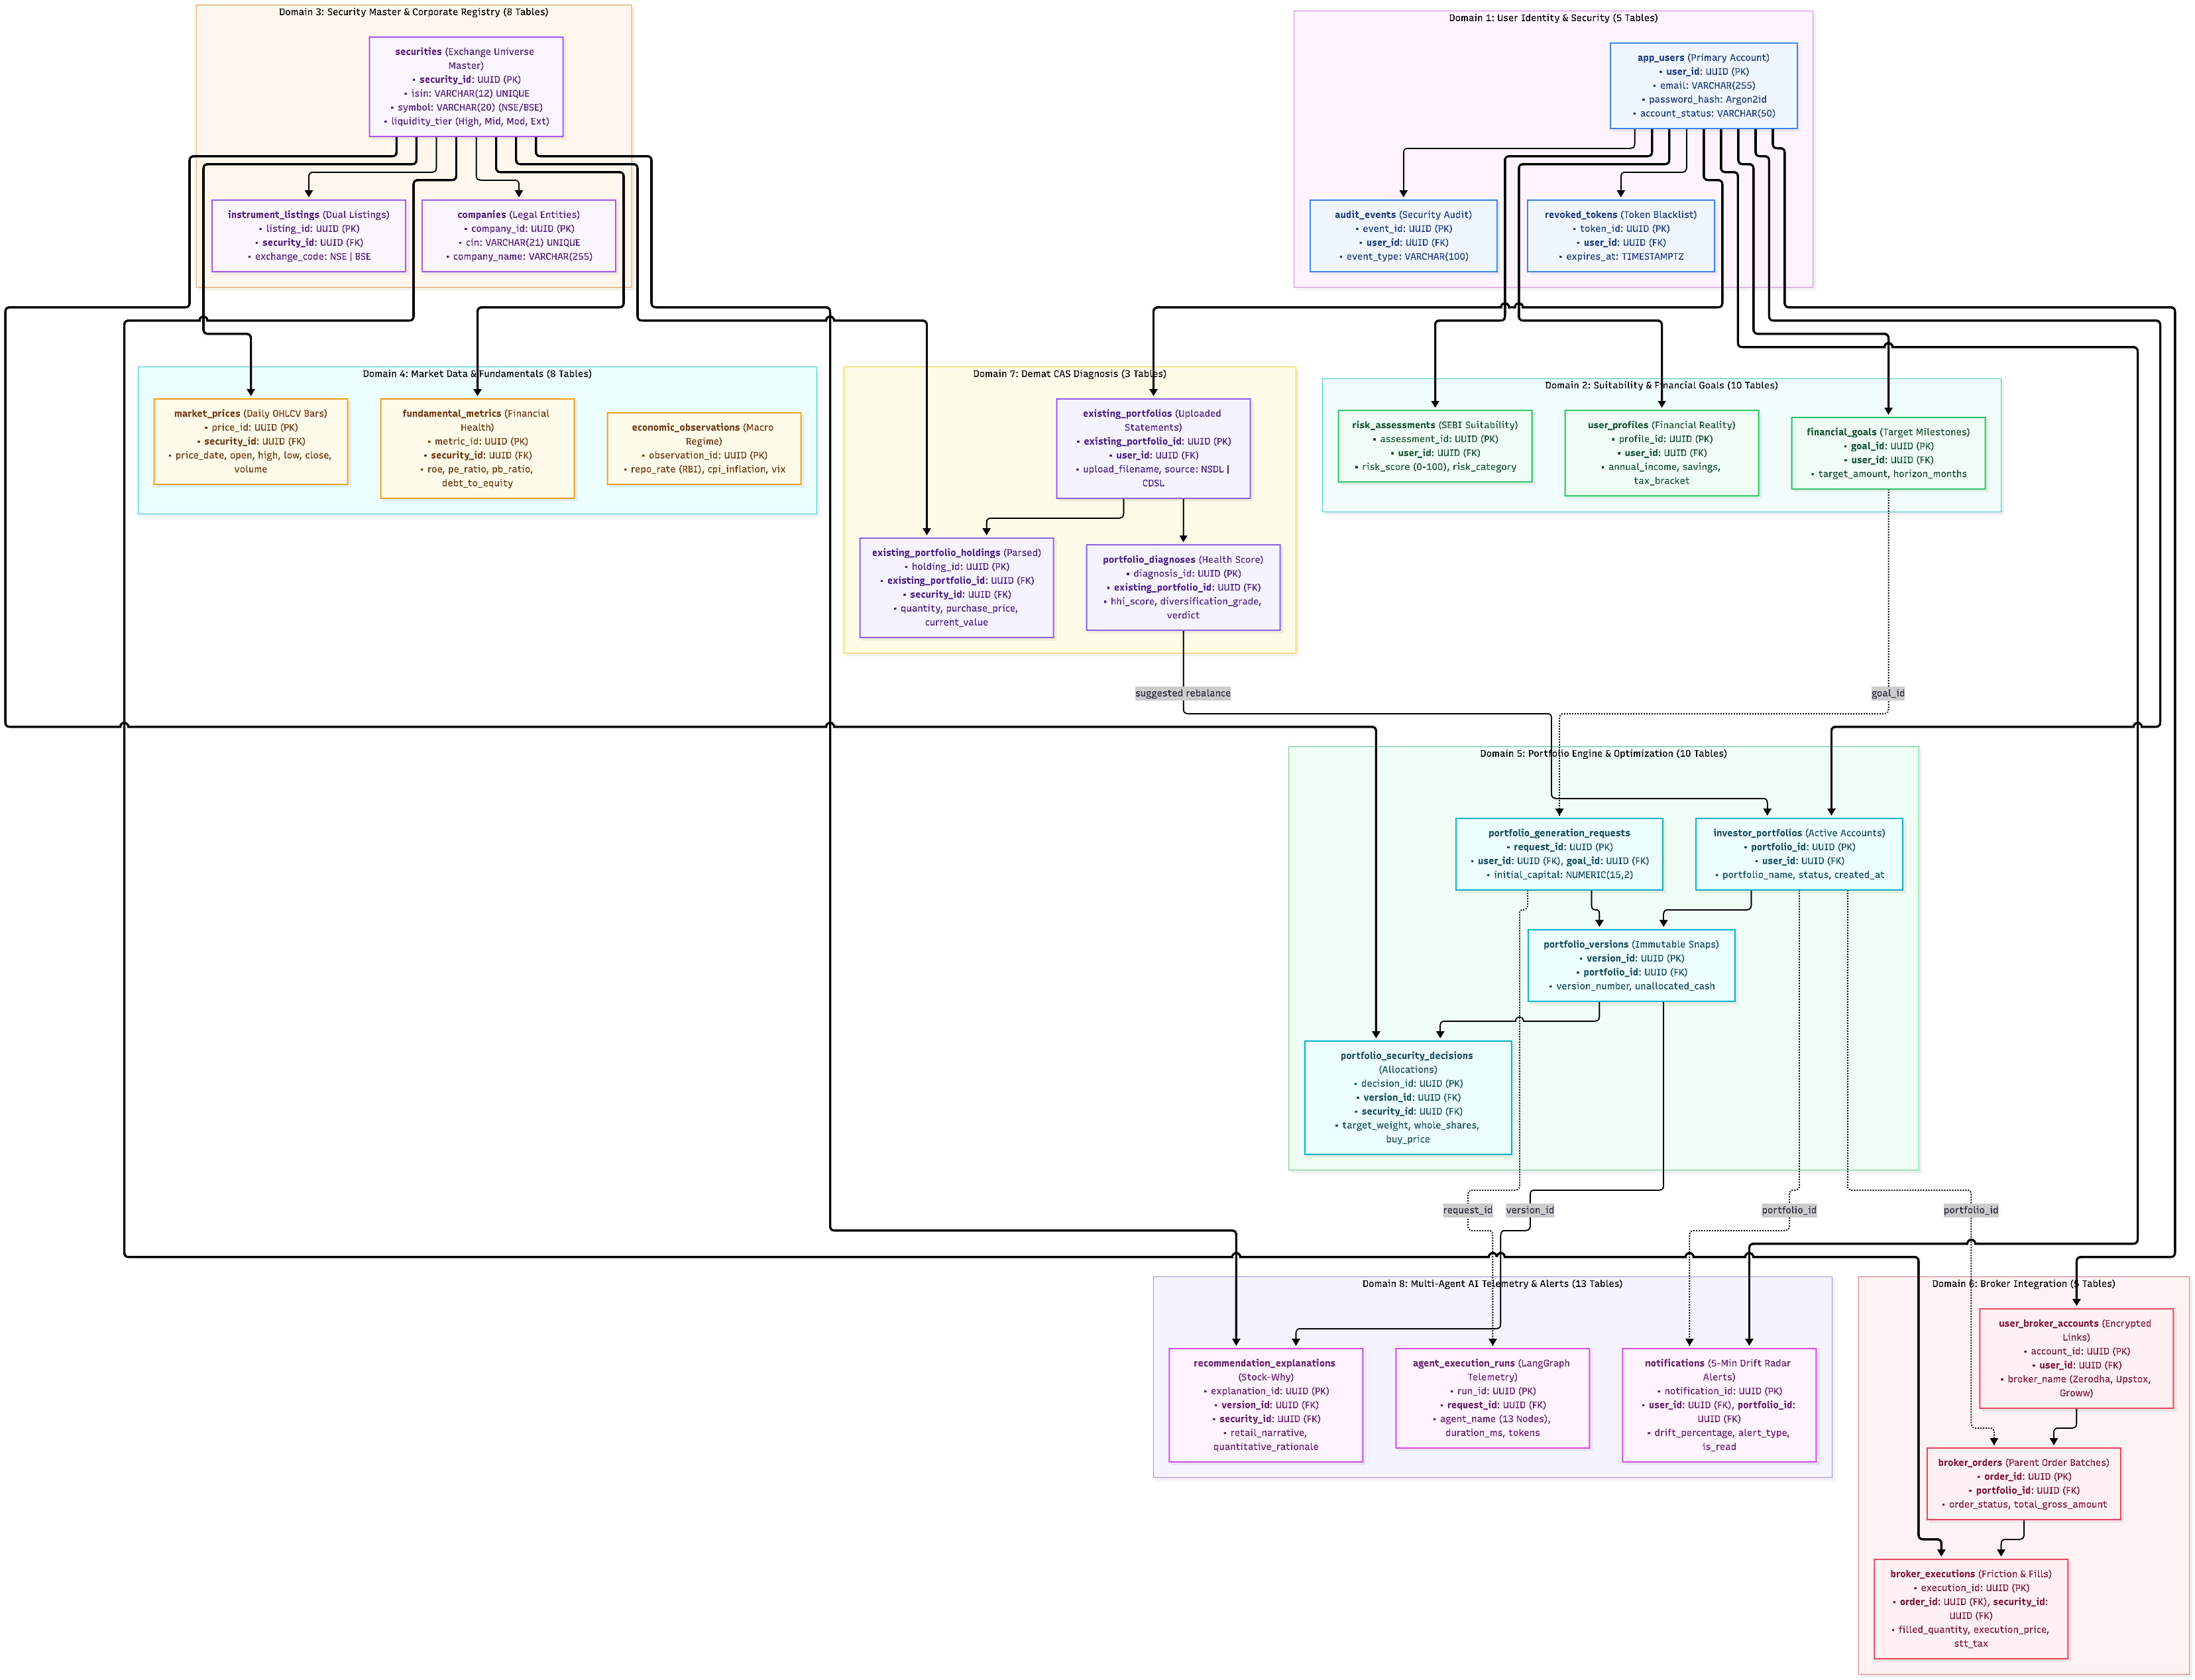
\includegraphics[width=\textwidth]{00_master_er_diagram.pdf}
    \caption{Lucid Master Database Entity-Relationship Diagram (63 Tables)}
    \label{fig:master_er}
\end{figure}

\section{Domain-Wise Schema Specifications}

\subsection{Domain 1: Identity, Authentication and Security Governance}
Domain 1 manages user authentication, enterprise cryptographic credentials, token blacklists, consent tracking, and security audit trails.

\begin{figure}[!htbp]
    \centering
    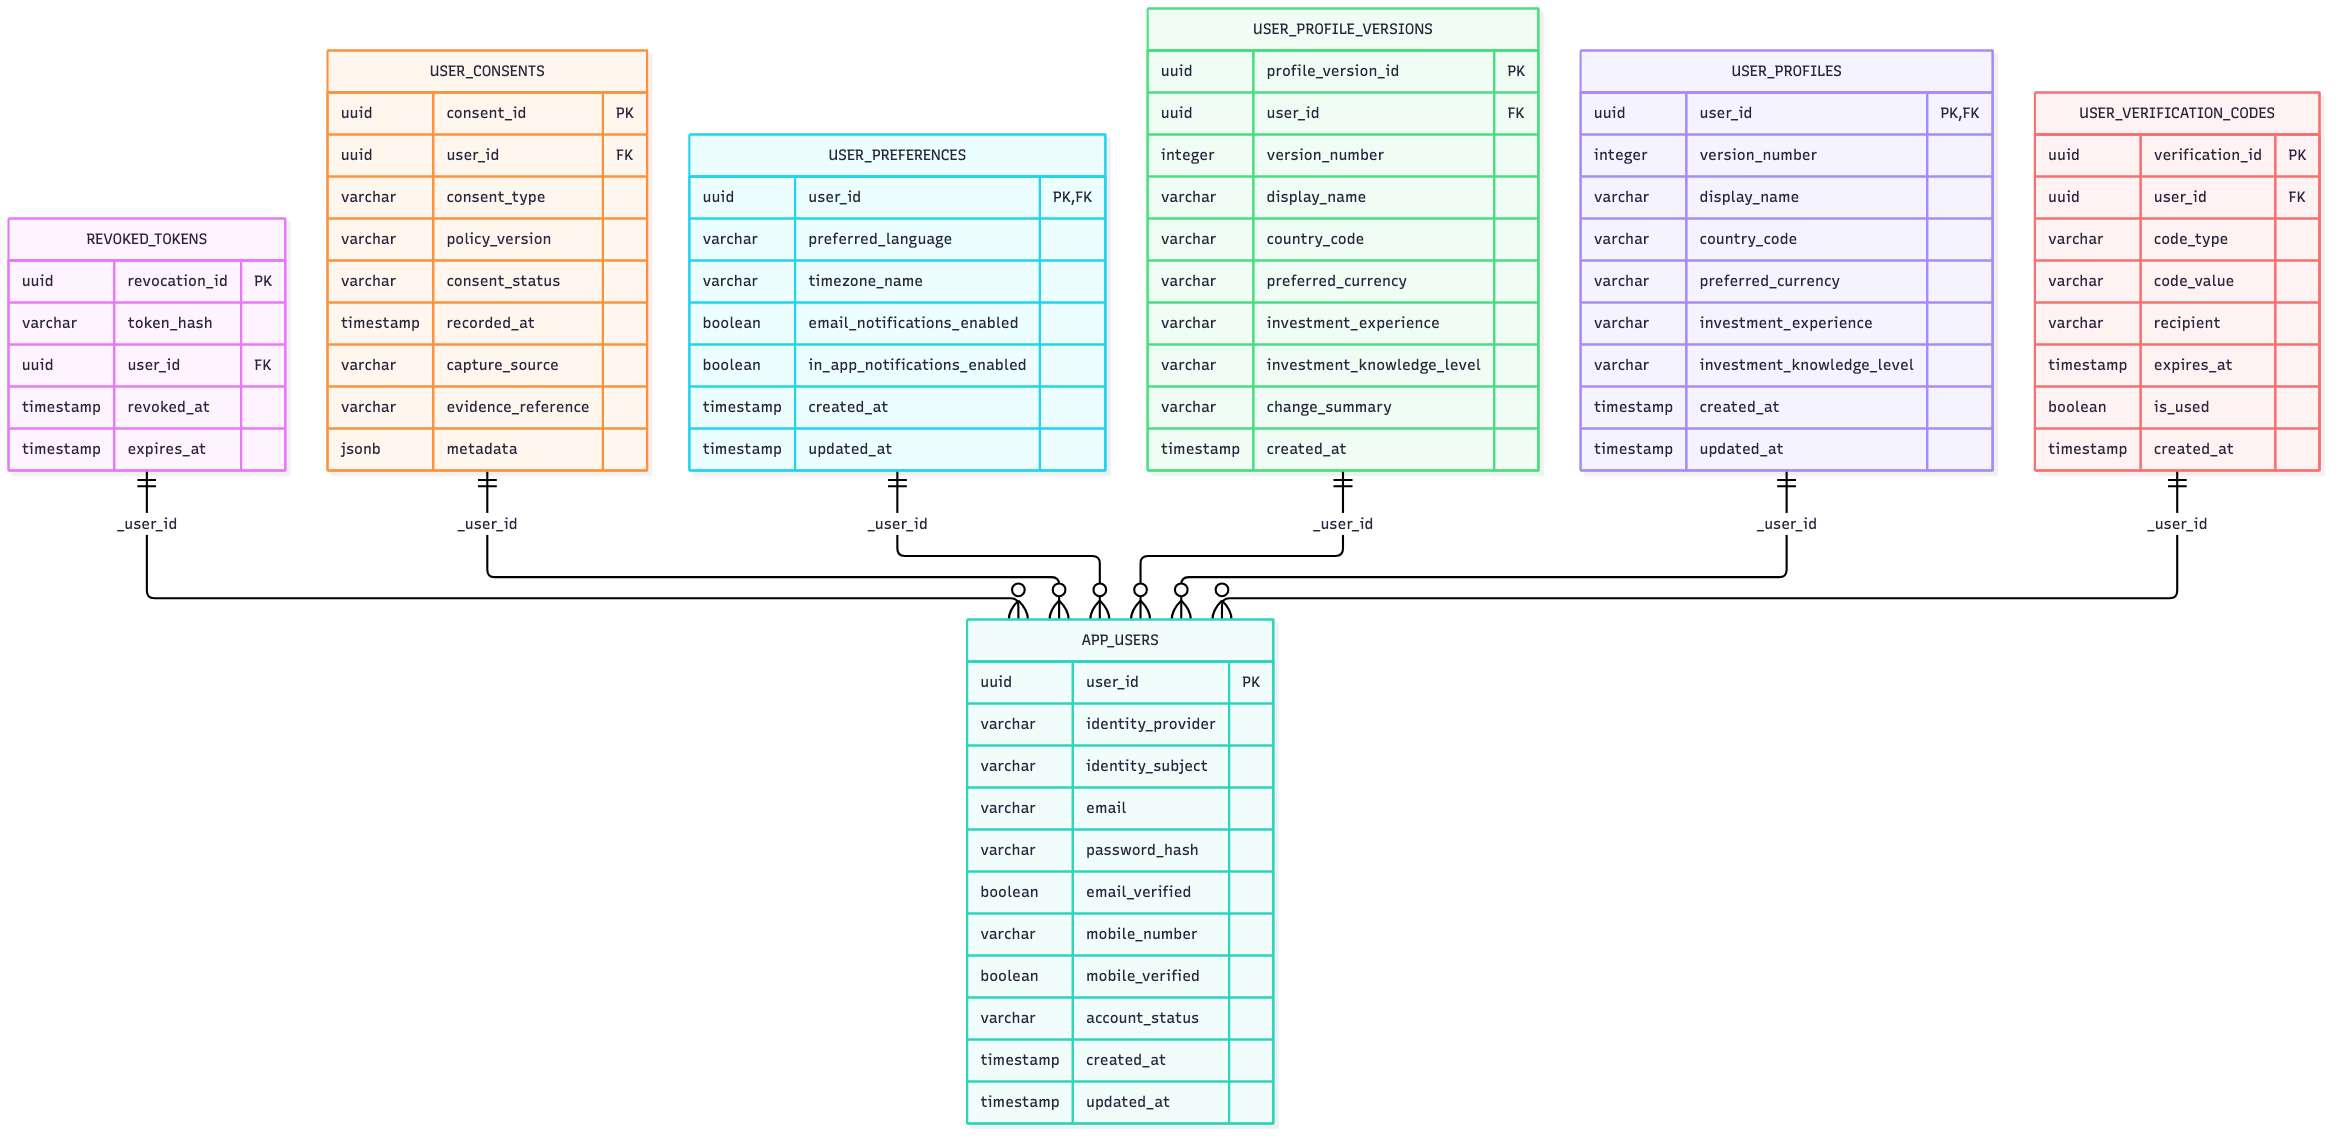
\includegraphics[width=0.88\textwidth, height=0.55\textheight, keepaspectratio]{01_identity_and_security_domain.png}
    \caption{Domain 1 ER Diagram: Identity, Authentication and Security Governance}
    \label{fig:er_domain1}
\end{figure}

\subsubsection{Table: \texttt{app\_users}}
The primary identity ledger storing registered investor accounts.
\begin{table}[H]
\centering
\caption{Schema Specification: \texttt{app\_users}}
\label{tab:schema_app_users}
\resizebox{\textwidth}{!}{%
\begin{tabular}{llcccl}
\toprule
\textbf{Column Name} & \textbf{Data Type} & \textbf{PK} & \textbf{FK} & \textbf{Nullable} & \textbf{Description \& Constraints} \\
\midrule
\texttt{user\_id} & \texttt{UUID} & Yes & No & No & Primary Key, generated via \texttt{uuid\_generate\_v4()} \\
\texttt{identity\_provider} & \texttt{VARCHAR(50)} & No & No & No & Auth provider (\texttt{local}, \texttt{google}, \texttt{apple}), default \texttt{'local'} \\
\texttt{identity\_subject} & \texttt{VARCHAR(255)} & No & No & No & Unique subject identifier from auth provider \\
\texttt{email} & \texttt{VARCHAR(255)} & No & No & No & Unique investor email address (indexed) \\
\texttt{password\_hash} & \texttt{VARCHAR(255)} & No & No & Yes & Canonical Argon2id cryptographic hash (RFC 9106) \\
\texttt{mobile\_number} & \texttt{VARCHAR(20)} & No & No & Yes & Investor contact number \\
\texttt{email\_verified} & \texttt{BOOLEAN} & No & No & No & Email verification flag (default \texttt{FALSE}) \\
\texttt{mobile\_verified} & \texttt{BOOLEAN} & No & No & No & Mobile verification flag (default \texttt{FALSE}) \\
\texttt{account\_status} & \texttt{VARCHAR(50)} & No & No & No & Status: \texttt{'active'}, \texttt{'suspended'}, \texttt{'pending'}, default \texttt{'active'} \\
\texttt{created\_at} & \texttt{TIMESTAMPTZ} & No & No & No & Record creation timestamp \\
\texttt{updated\_at} & \texttt{TIMESTAMPTZ} & No & No & No & Last update timestamp \\
\bottomrule
\end{tabular}%
}
\end{table}

\noindent \textbf{Additional Domain 1 Tables}:
\begin{itemize}
    \item \texttt{revoked\_tokens}: Stores invalidated JWT token signatures (\texttt{jti} UUID, expiry timestamp) to enforce immediate logout.
    \item \texttt{user\_consents}: Tracks SEBI risk disclosures, terms of service, and privacy policy agreements (\texttt{consent\_type}, \texttt{version}, \texttt{ip\_address}).
    \item \texttt{user\_verification\_codes}: Manages time-limited OTP tokens for email and mobile phone verification (\texttt{code\_hash}, \texttt{expires\_at}).
    \item \texttt{audit\_events}: Tamper-evident ledger capturing security events, login attempts, password changes, and administrative actions (\texttt{event\_type}, \texttt{actor\_id}, \texttt{details\_json}).
\end{itemize}

\clearpage
\subsection{Domain 2: Investor Suitability, Profiling and Financial Goals}
Domain 2 captures the investor's financial reality, investment horizon, psychometric risk tolerance, and life goals across 10 specialized tables:

\begin{itemize}
    \item \texttt{user\_profiles}: Investor demographic and financial data (monthly income, investment horizon, net worth, tax bracket).
    \item \texttt{user\_profile\_versions}: Historical audit versions of investor profiles tracking changes over time.
    \item \texttt{financial\_goals}: Explicit investor milestones (\texttt{goal\_type}: wealth accumulation, retirement, child education; target corpus, target date).
    \item \texttt{user\_preferences}: General UI, notification, and currency preferences.
    \item \texttt{risk\_questions}: Canonical bank of SEBI suitability questions (\texttt{question\_text}, \texttt{category}, \texttt{weight}).
    \item \texttt{risk\_question\_options}: Scored answer choices per question (\texttt{option\_text}, \texttt{score\_points}).
    \item \texttt{risk\_assessments}: Assessment execution header (\texttt{user\_id}, \texttt{total\_score}, \texttt{risk\_category}: conservative, moderate, aggressive).
    \item \texttt{risk\_assessment\_answers}: Investor selections mapping to specific question options.
    \item \texttt{user\_security\_preferences}: Explicit stock-level inclusion or exclusion mandates (\texttt{ticker}, \texttt{preference\_type}: MANDATORY\_INCLUDE, EXCLUDE).
    \item \texttt{user\_sector\_preferences}: Sector-level preferences (e.g., exclude tobacco, defense, or real estate).
\end{itemize}

Figure~\ref{fig:er_domain2} illustrates the Entity-Relationship schema for Domain 2:

\begin{figure}[!htbp]
    \centering
    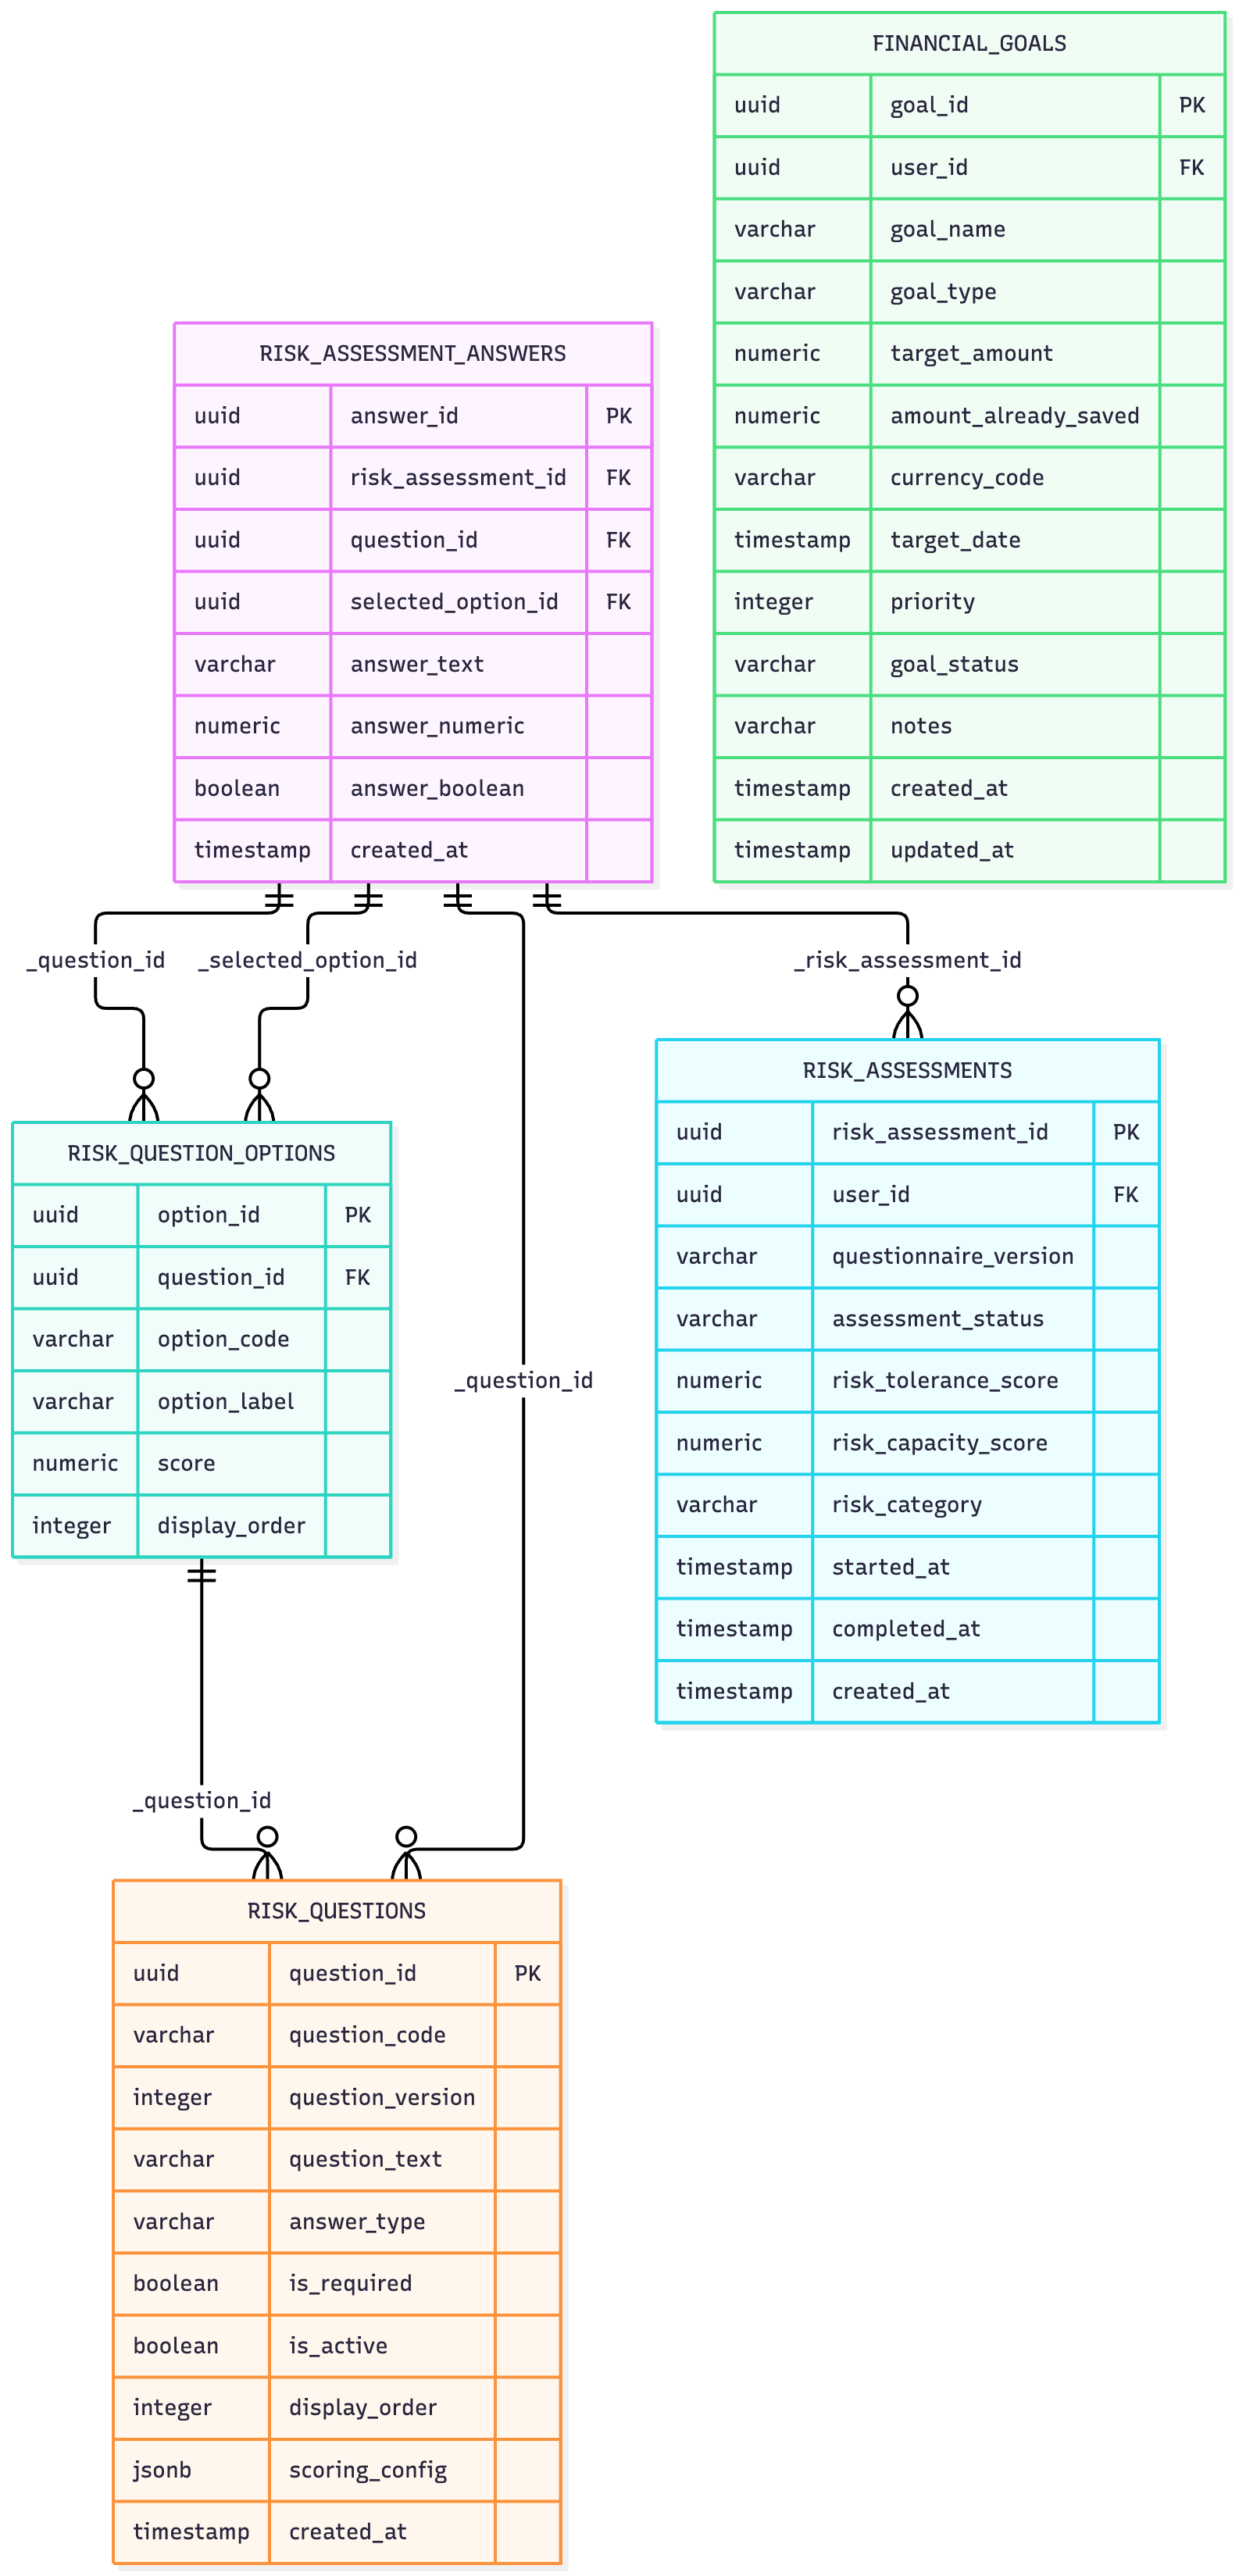
\includegraphics[width=0.88\textwidth, height=0.48\textheight, keepaspectratio]{02_investor_suitability_and_goals_domain.png}
    \caption{Domain 2 ER Diagram: Investor Suitability, Profiling and Financial Goals}
    \label{fig:er_domain2}
\end{figure}

\clearpage
\subsection{Domain 3: Security Master and Corporate Registry}
Domain 3 defines the financial market universe, listed equities, exchanges, sectors, and cross-exchange ticker mappings across 8 tables:

\begin{itemize}
    \item \texttt{exchanges}: Exchange directory (\texttt{exchange\_code}: NSE, BSE; country, operating currency).
    \item \texttt{sectors}: Macro-economic sectors (Financial Services, IT, Healthcare, FMCG, Energy).
    \item \texttt{industries}: Granular industry taxonomy mapped to parent sectors.
    \item \texttt{companies}: Corporate issuers (\texttt{cin\_number}, \texttt{company\_name}, \texttt{incorporation\_date}).
    \item \texttt{company\_industries}: Junction table enabling multi-industry corporate classification.
    \item \texttt{securities}: Canonical equity master (\texttt{security\_id}, \texttt{isin} [Unique], \texttt{company\_id}, \texttt{security\_type}: EQUITY, \texttt{liquidity\_tier}).
    \item \texttt{instrument\_listings}: Exchange-specific trading listings (\texttt{security\_id}, \texttt{exchange\_id}, \texttt{ticker\_symbol}, e.g., RELIANCE on NSE vs 500325 on BSE).
    \item \texttt{source\_instrument\_mappings}: Maps exchange tickers to external API identifiers (Yahoo Finance tickers, e.g., \texttt{RELIANCE.NS}).
\end{itemize}

Figure~\ref{fig:er_domain3} illustrates the Entity-Relationship schema for Domain 3:

\begin{figure}[!htbp]
    \centering
    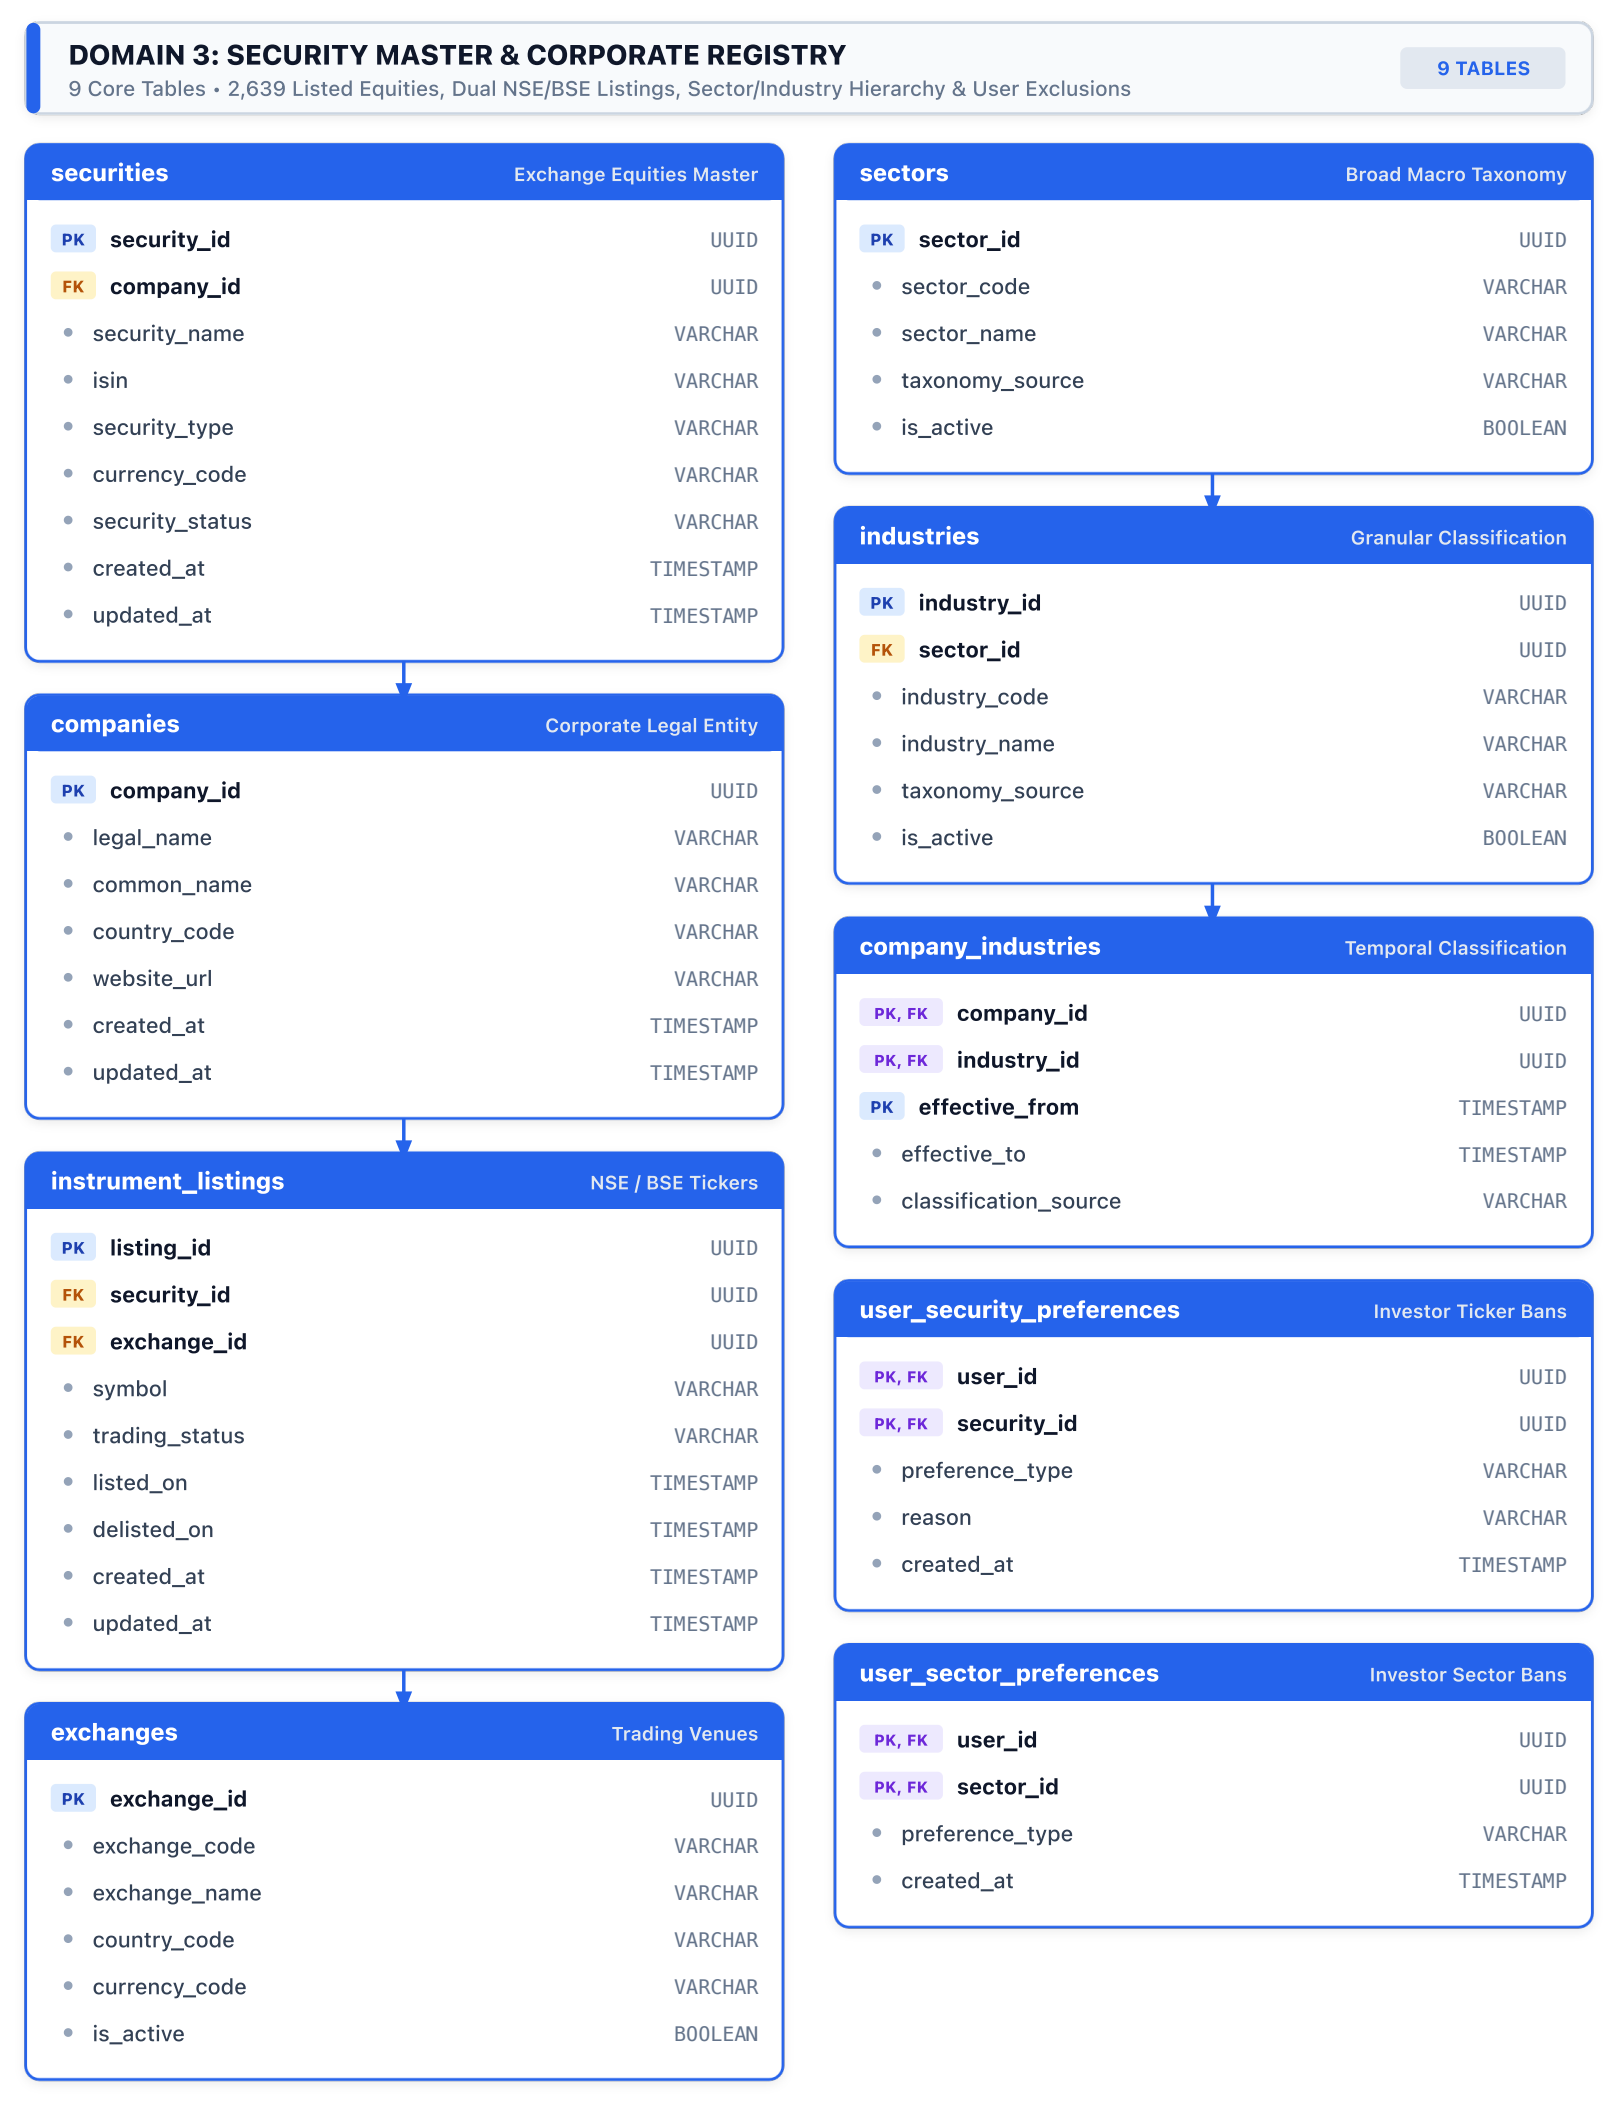
\includegraphics[width=0.88\textwidth, height=0.50\textheight, keepaspectratio]{03_security_master_and_companies_domain.png}
    \caption{Domain 3 ER Diagram: Security Master and Corporate Registry}
    \label{fig:er_domain3}
\end{figure}

\clearpage
\subsection{Domain 4: Market Data, Historical Quotes and Macro Regime}
Domain 4 stores historical pricing, corporate fundamentals, macroeconomic indicators, and financial news across 8 tables:

\begin{itemize}
    \item \texttt{market\_prices}: Daily historical OHLCV records (\texttt{security\_id}, \texttt{price\_date}, \texttt{open}, \texttt{high}, \texttt{low}, \texttt{close}, \texttt{adj\_close}, \texttt{volume}).
    \item \texttt{fundamental\_metrics}: Point-in-time balance sheet metrics (\texttt{security\_id}, \texttt{period\_end}, \texttt{pe\_ratio}, \texttt{pb\_ratio}, \texttt{roe\_pct}, \texttt{debt\_to\_equity}, \texttt{market\_cap}).
    \item \texttt{metric\_definitions}: Metadata catalog defining calculation formulas and units for financial metrics.
    \item \texttt{economic\_indicators}: Macroeconomic series definitions (RBI Repo Rate, CPI Inflation, India 10Y Bond Yield).
    \item \texttt{economic\_observations}: Point-in-time observations for macroeconomic indicators.
    \item \texttt{market\_news\_articles}: Ingested financial news articles (\texttt{headline}, \texttt{content}, \texttt{published\_at}, \texttt{sentiment\_score}).
    \item \texttt{news\_article\_securities}: Junction table mapping articles to specific security ISINs.
    \item \texttt{knowledge\_documents}: Regulatory circulars and investment knowledge artifacts.
\end{itemize}

Figure~\ref{fig:er_domain4} illustrates the Entity-Relationship schema for Domain 4:

\begin{figure}[!htbp]
    \centering
    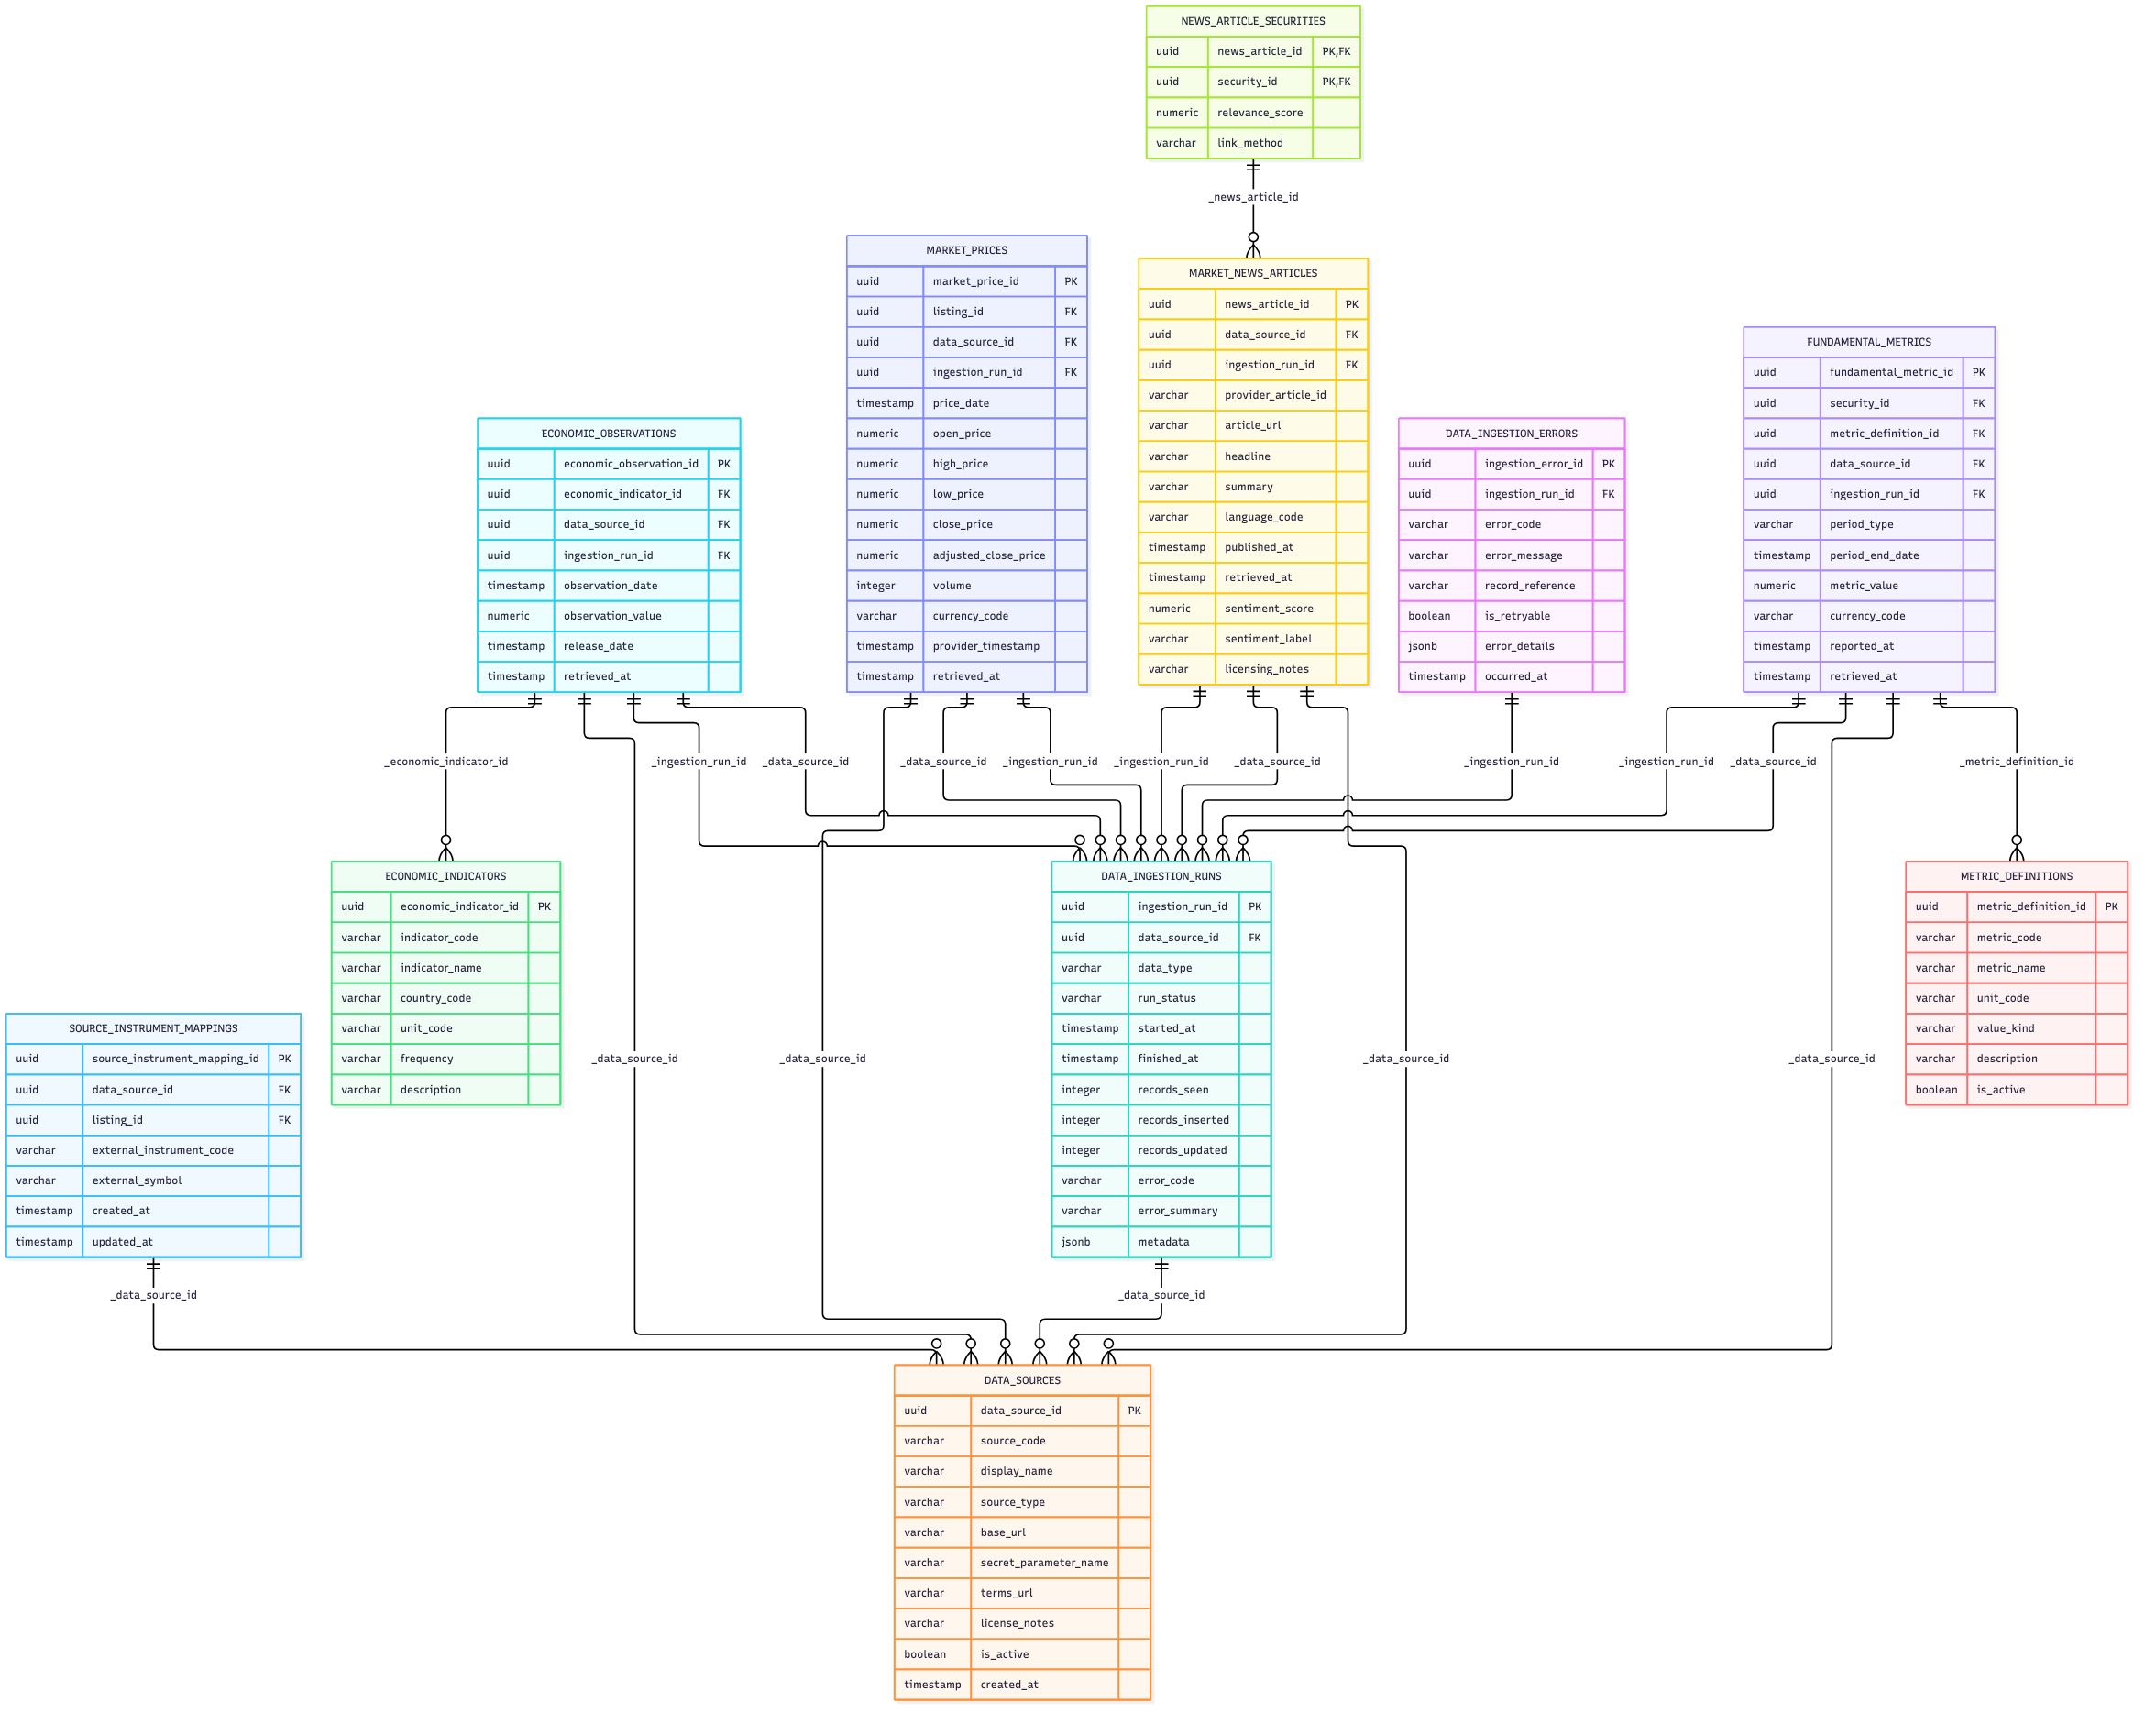
\includegraphics[width=0.88\textwidth, height=0.50\textheight, keepaspectratio]{04_market_data_and_fundamentals_domain.png}
    \caption{Domain 4 ER Diagram: Market Data, Historical Quotes and Macro Regime}
    \label{fig:er_domain4}
\end{figure}

\clearpage
\subsection{Domain 5: Portfolio Engine, Quantitative Optimization and Tracking}
Domain 5 forms the transactional core of Lucid, recording recommended portfolios, versioned weight distributions, and performance snapshots across 10 tables:

\begin{itemize}
    \item \texttt{strategy\_definitions}: Core strategy templates (Conservative Income, Moderate Balanced, Aggressive Growth).
    \item \texttt{strategy\_versions}: Versioned mathematical parameter sets per strategy.
    \item \texttt{investor\_portfolios}: Master portfolio container per user (\texttt{portfolio\_id}, \texttt{user\_id}, \texttt{portfolio\_status}: active, archived).
    \item \texttt{portfolio\_versions}: Immutable version snapshots (\texttt{version\_number}, \texttt{rebalance\_reason}, \texttt{effective\_date}, \texttt{cash\_balance}).
    \item \texttt{portfolio\_version\_constraints}: Exact mathematical bounds applied to a version (max single stock 25\%, max sector 40\%).
    \item \texttt{portfolio\_generation\_requests}: Ingested generation telemetry capturing user input parameters.
    \item \texttt{portfolio\_security\_decisions}: Line-item security allocations (\texttt{security\_id}, \texttt{target\_weight\_pct}, \texttt{allocated\_shares}, \texttt{buy\_price}, \texttt{allocated\_amount}).
    \item \texttt{portfolio\_performance\_snapshots}: Daily NAV records tracking equity value and cumulative returns.
    \item \texttt{portfolio\_scenarios}: Stress-testing projections evaluating portfolio resilience under historical shocks.
    \item \texttt{rebalance\_suggestions}: Proposed rebalancing actions generated by the monitoring engine.
\end{itemize}

Figure~\ref{fig:er_domain5} illustrates the Entity-Relationship schema for Domain 5:

\begin{figure}[!htbp]
    \centering
    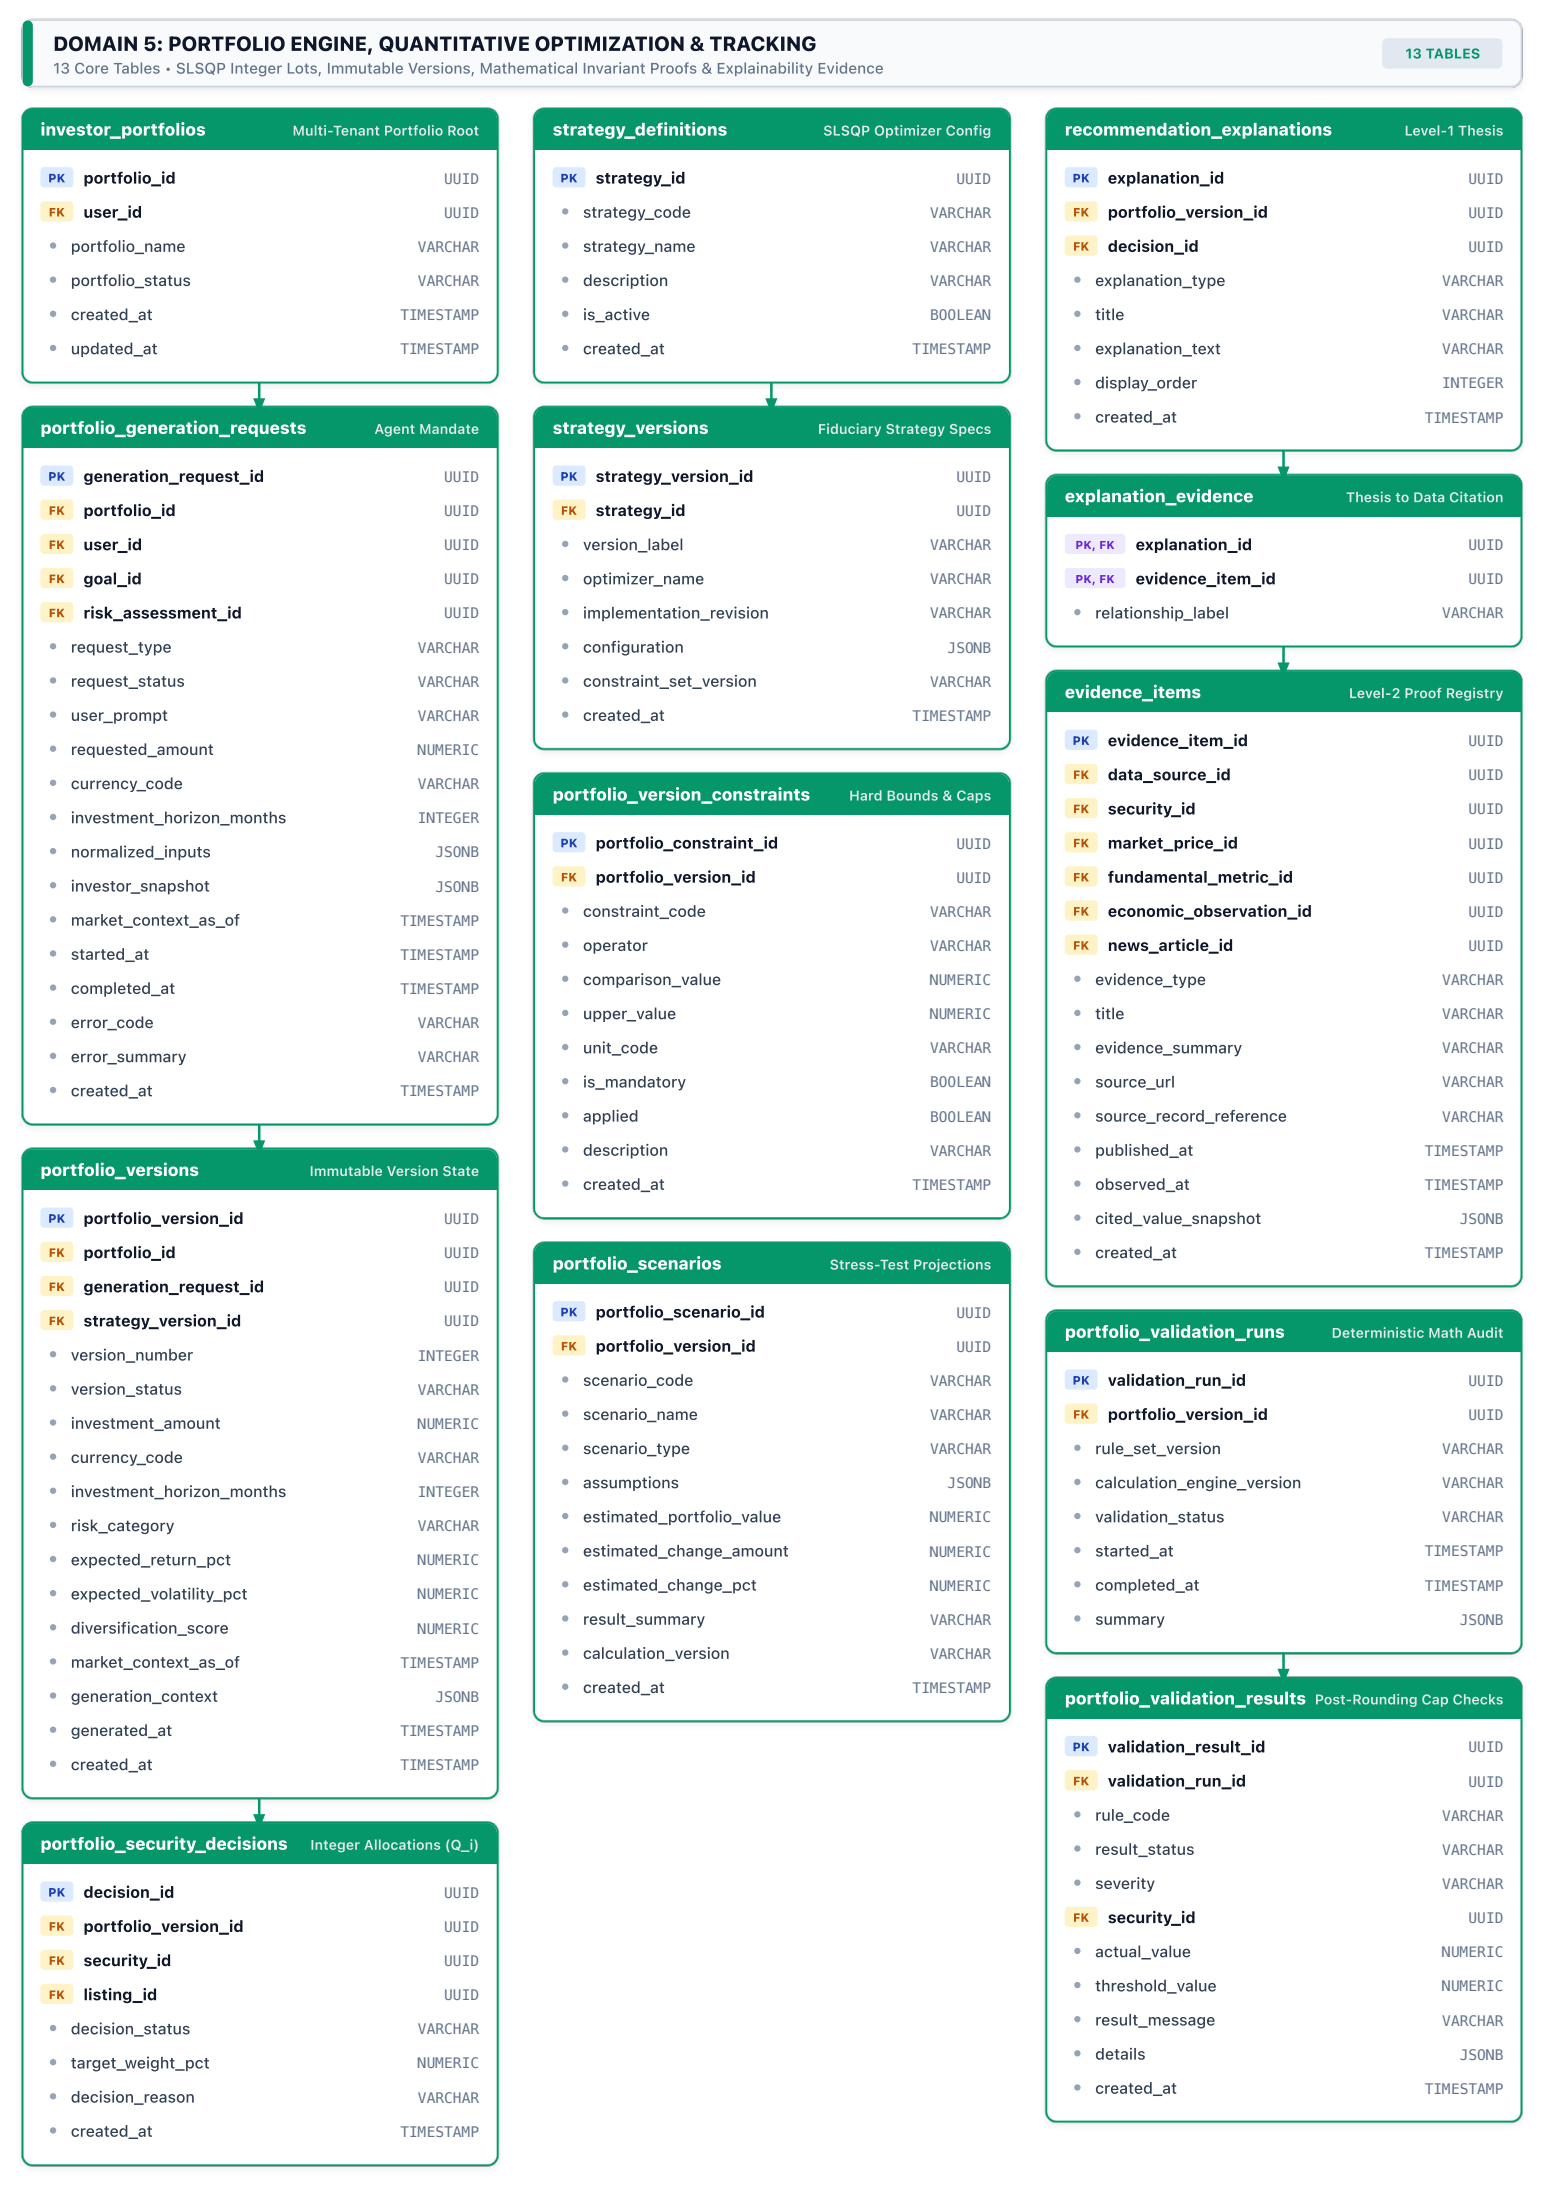
\includegraphics[width=0.88\textwidth, height=0.48\textheight, keepaspectratio]{05_portfolio_engine_and_optimization_domain.png}
    \caption{Domain 5 ER Diagram: Portfolio Engine, Quantitative Optimization and Tracking}
    \label{fig:er_domain5}
\end{figure}

\clearpage
\subsection{Domain 6: Broker Integration, Execution and Order Lifecycle}
Domain 6 manages demat broker connections, order generation, and simulated trade execution across 5 tables:

\begin{itemize}
    \item \texttt{broker\_providers}: Supported broker platforms (Zerodha, Upstox, Groww mock adapters).
    \item \texttt{user\_broker\_accounts}: User-linked broker accounts (\texttt{account\_status}, \texttt{api\_token\_encrypted}).
    \item \texttt{broker\_orders}: Parent order batches generated from portfolio rebalancing.
    \item \texttt{broker\_order\_events}: Lifecycle audit events per order (CREATED, SUBMITTED, EXECUTED, REJECTED).
    \item \texttt{broker\_executions}: Line-item execution records (\texttt{shares\_filled}, \texttt{average\_price}, \texttt{execution\_timestamp}).
\end{itemize}

Figure~\ref{fig:er_domain6} illustrates the Entity-Relationship schema for Domain 6:

\begin{figure}[H]
    \centering
    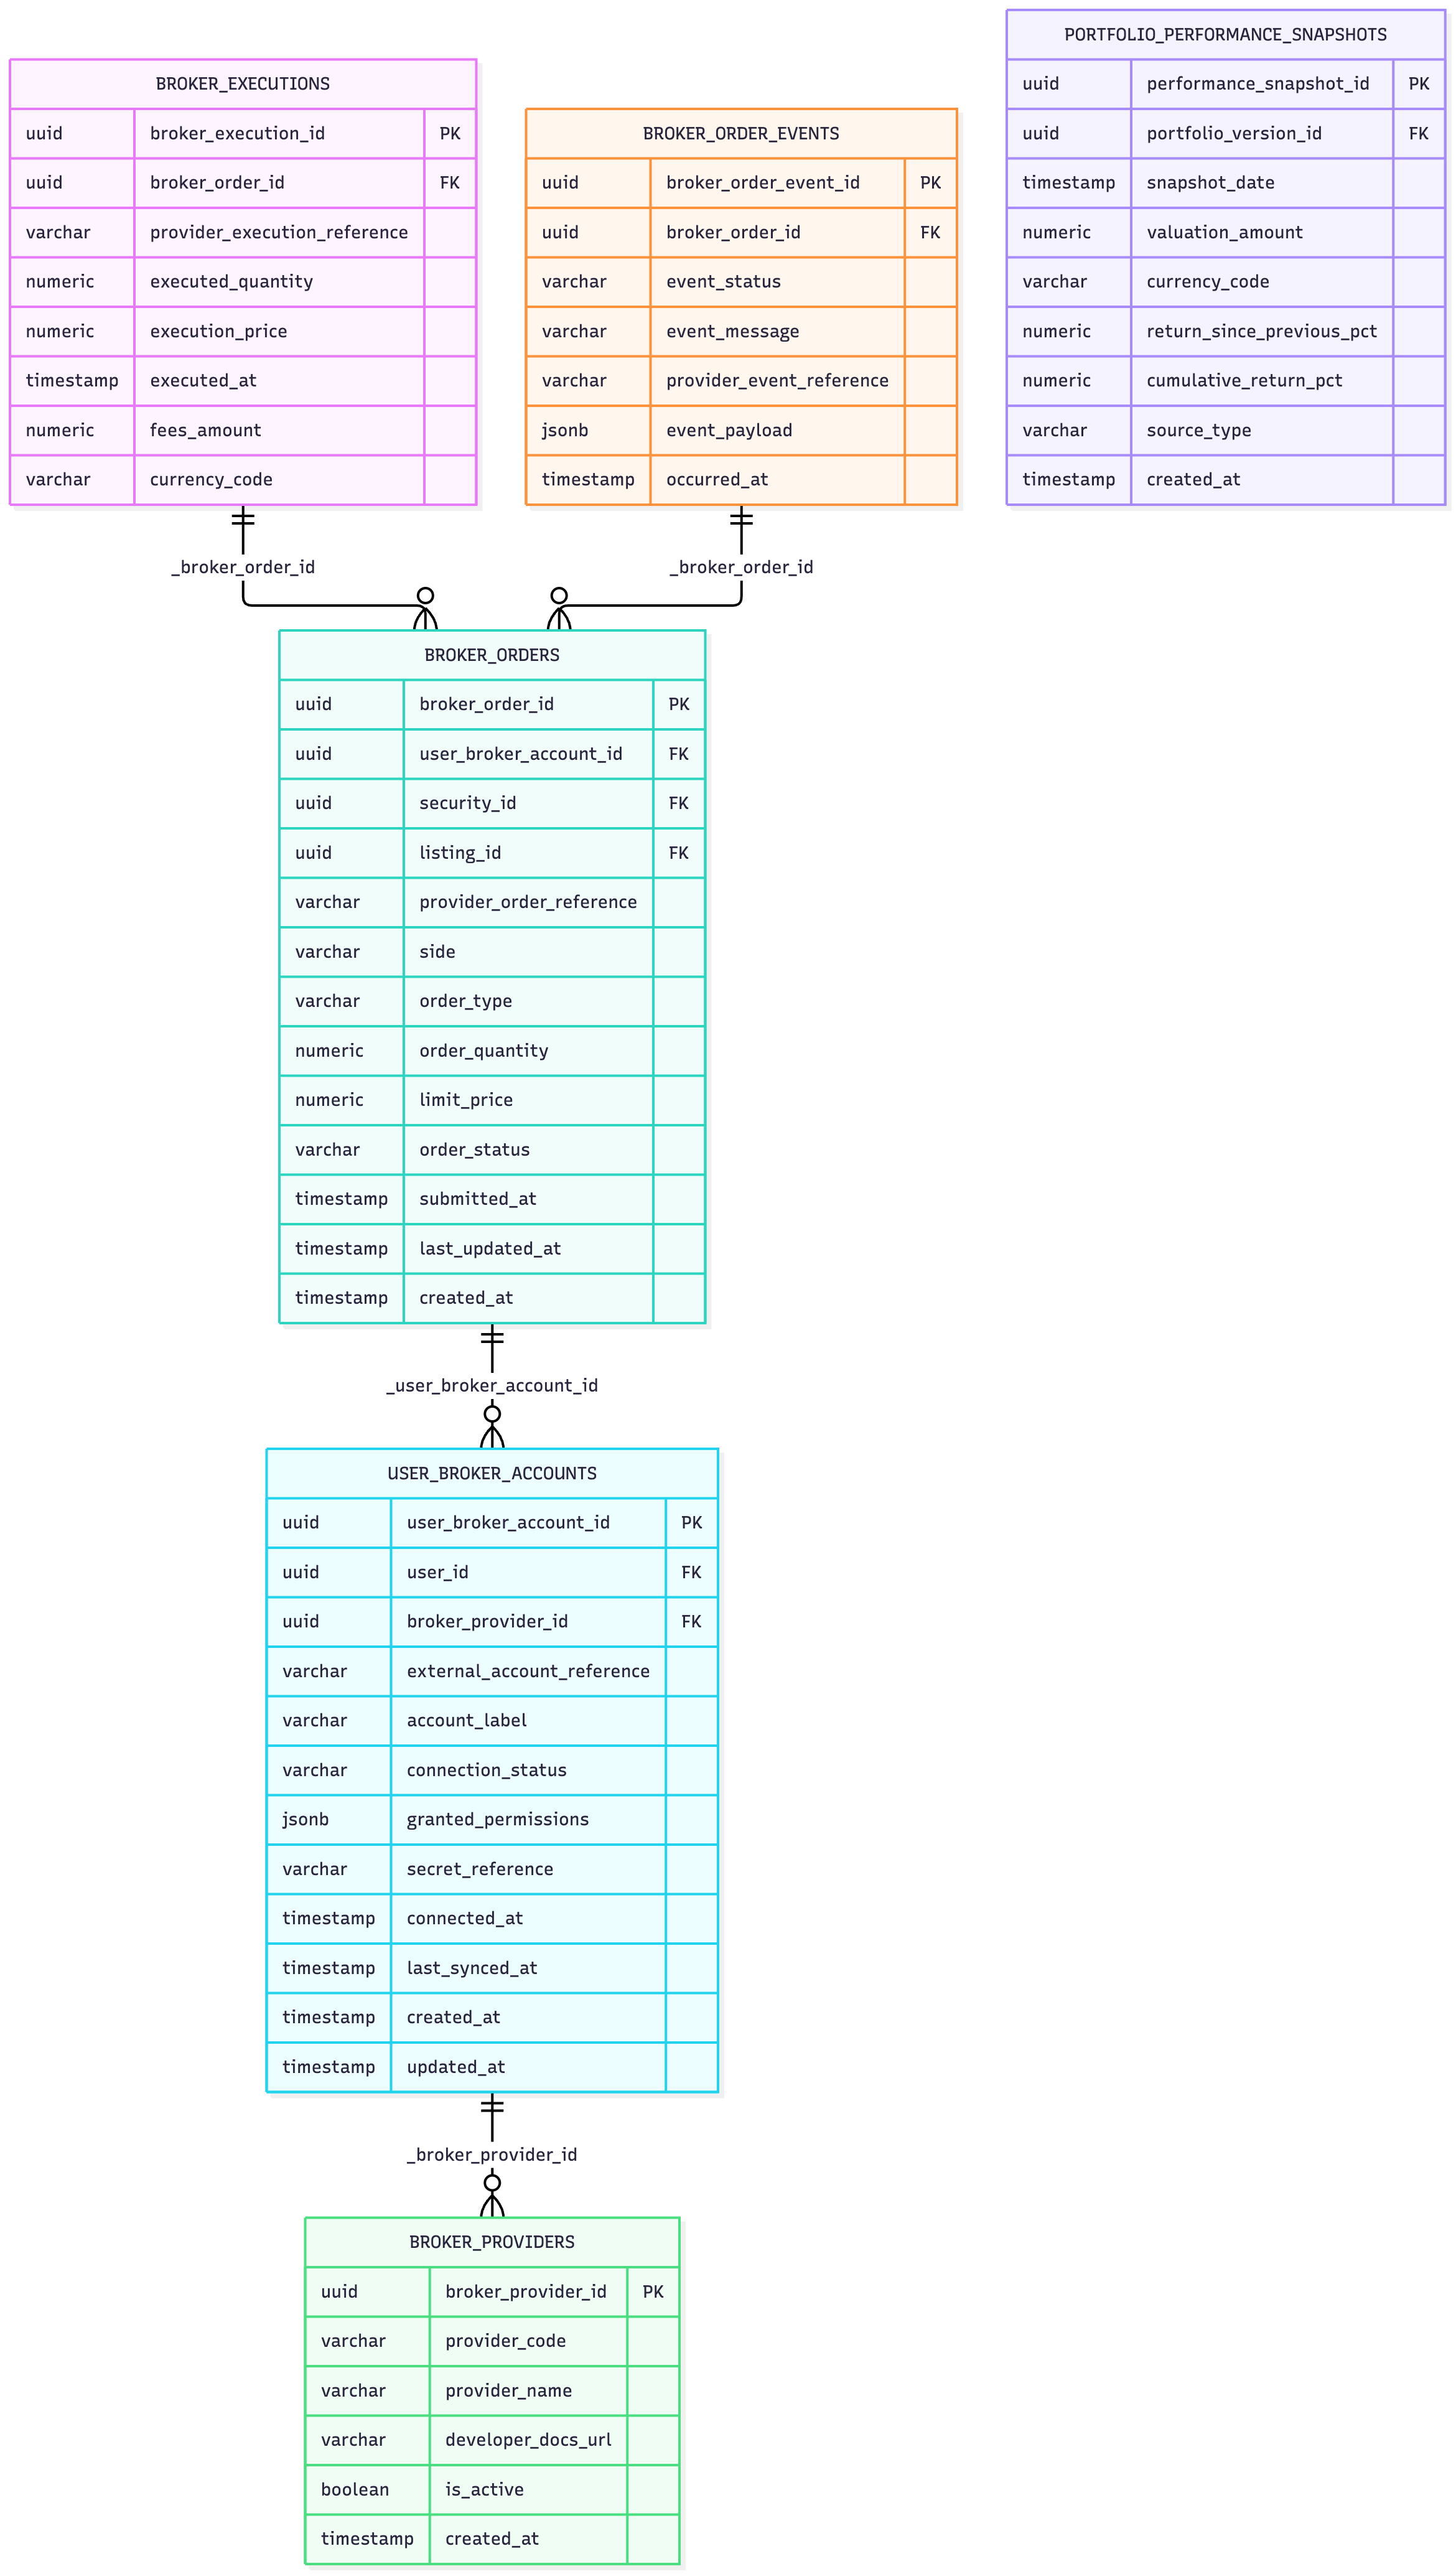
\includegraphics[width=0.88\textwidth, height=0.38\textheight, keepaspectratio]{06_broker_integrations_and_orders_domain.png}
    \caption{Domain 6 ER Diagram: Broker Integration, Execution and Order Lifecycle}
    \label{fig:er_domain6}
\end{figure}

\clearpage
\subsection{Domain 7: Demat CAS Diagnosis and Portfolio Analytics}
Domain 7 stores imported external Demat portfolios and health diagnostic assessments across 3 tables:

\begin{itemize}
    \item \texttt{existing\_portfolios}: Imported portfolio records (\texttt{source\_type}: CAS\_PDF, MANUAL\_ENTRY; upload timestamp).
    \item \texttt{existing\_portfolio\_holdings}: Parsed stock holdings (\texttt{isin}, \texttt{quantity}, \texttt{average\_buy\_price}, \texttt{current\_value}).
    \item \texttt{portfolio\_diagnoses}: Comprehensive diagnosis output (\texttt{hhi\_score}, \texttt{concentration\_risk\_level}, \texttt{sector\_skews\_json}, \texttt{recommendation\_summary}).
\end{itemize}

Figure~\ref{fig:er_domain7} illustrates the Entity-Relationship schema for Domain 7:

\begin{figure}[H]
    \centering
    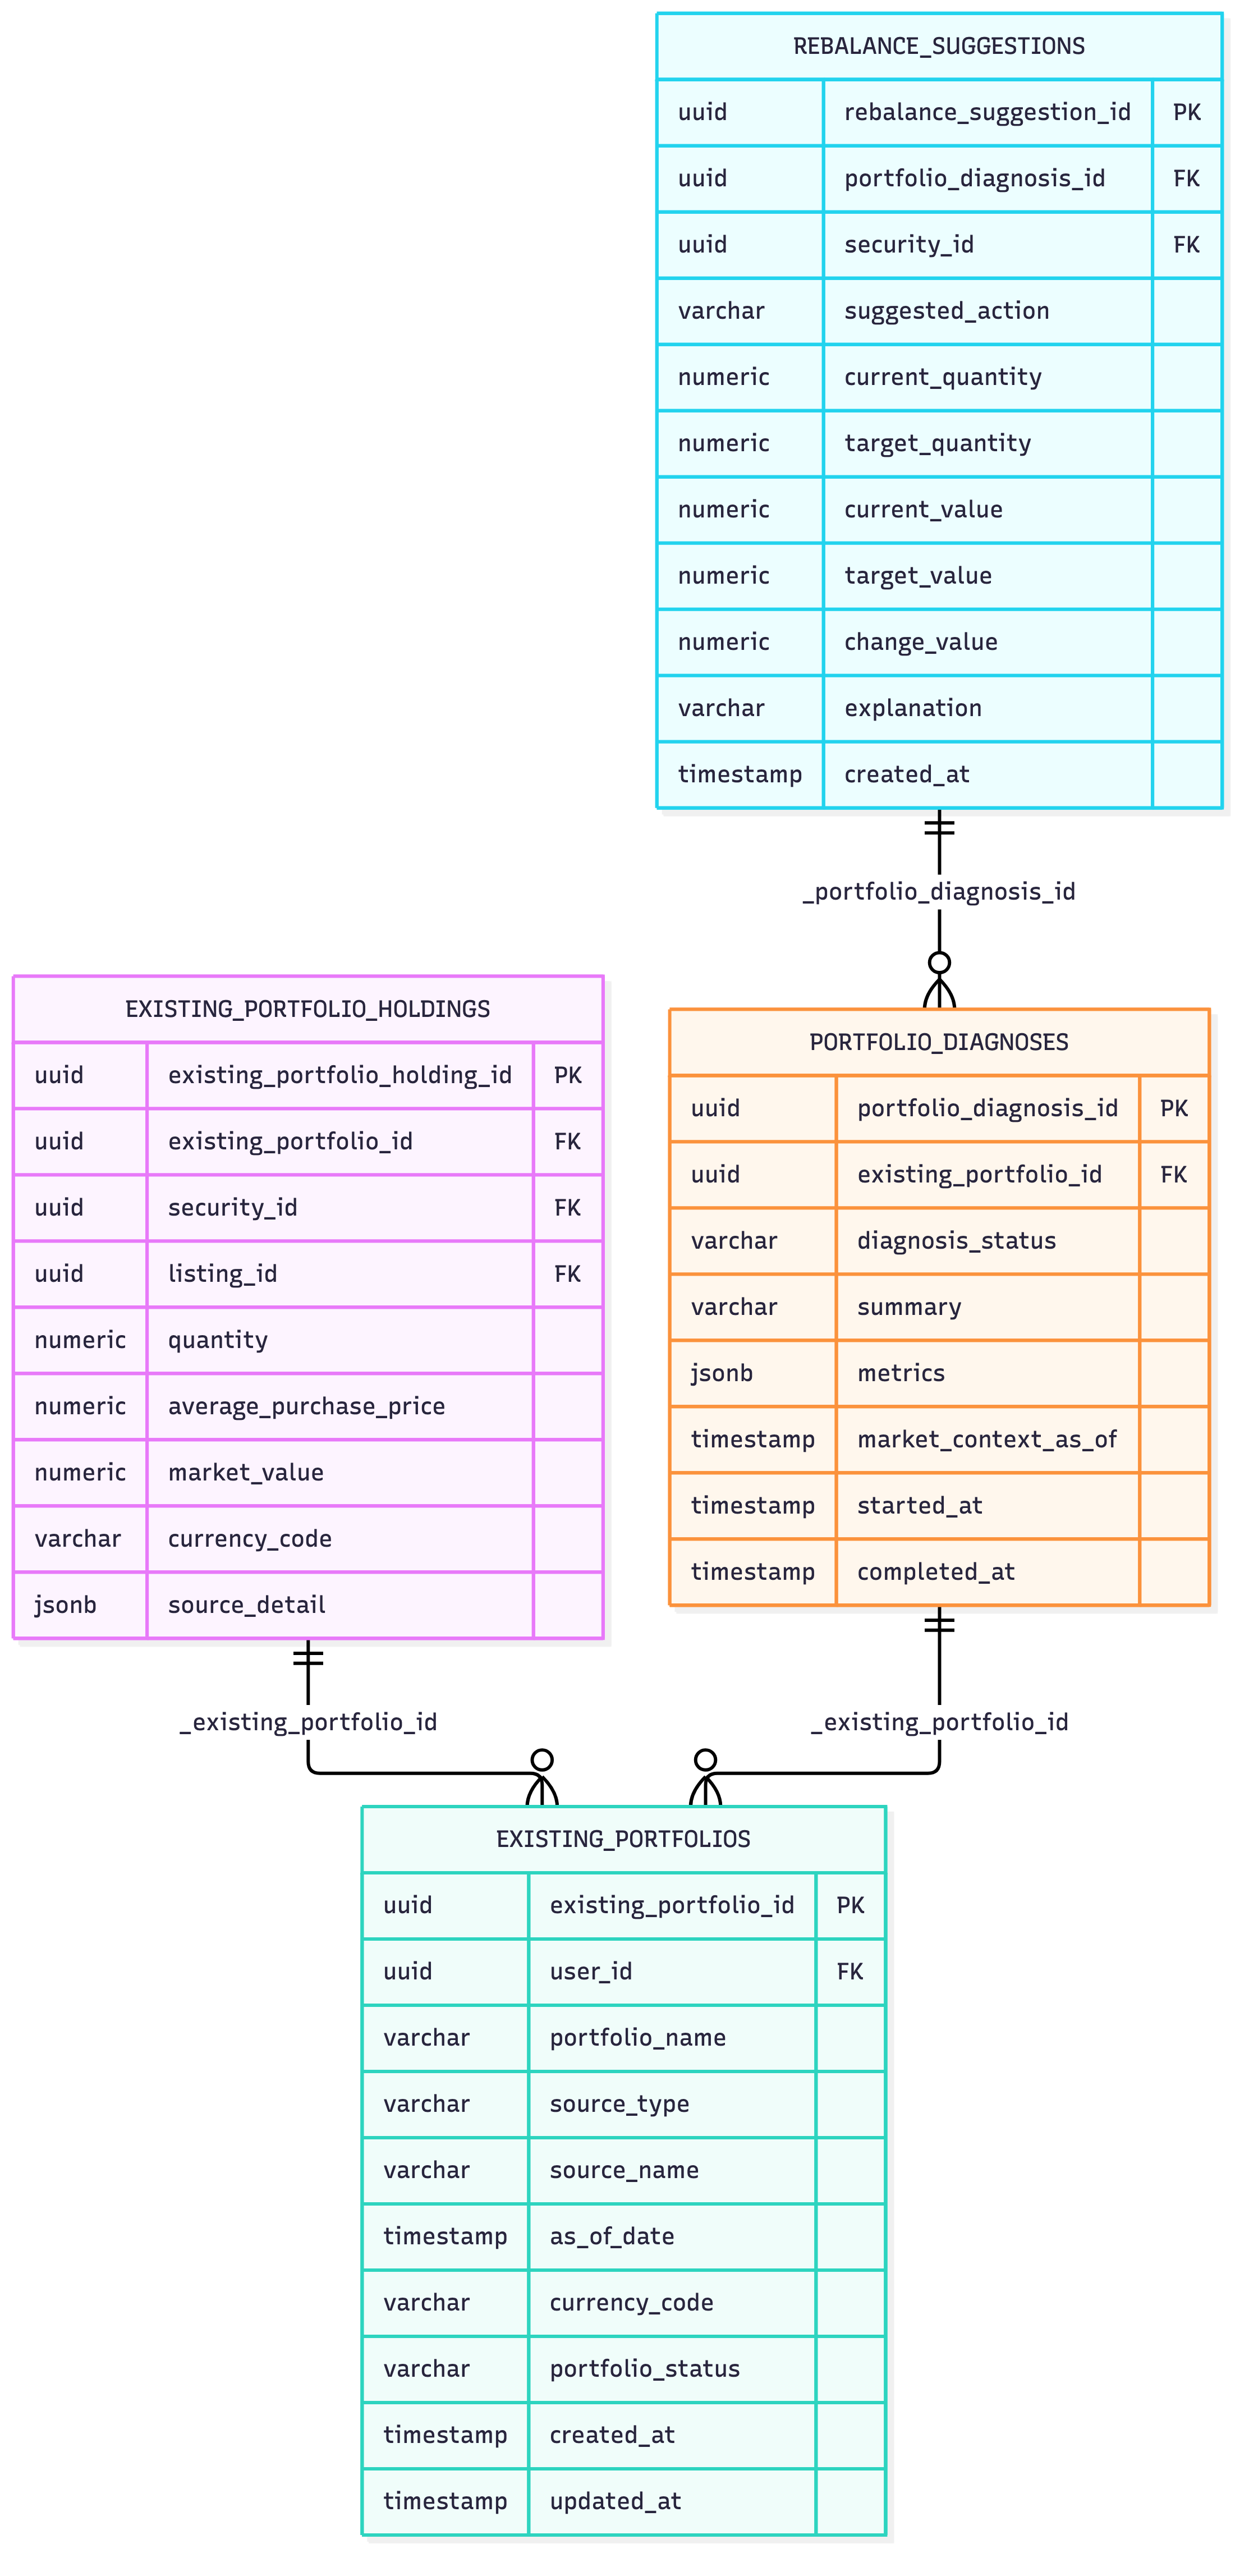
\includegraphics[width=0.88\textwidth, height=0.48\textheight, keepaspectratio]{07_demat_diagnosis_and_rebalancing_domain.png}
    \caption{Domain 7 ER Diagram: Demat CAS Diagnosis and Portfolio Analytics}
    \label{fig:er_domain7}
\end{figure}

\clearpage
\subsection{Domain 8: Multi-Agent AI Telemetry, Reasoning Traces and Verification}
Domain 8 captures LangGraph agent executions, fiduciary explanations, constraint verification runs, and notifications across 13 tables:

\begin{itemize}
    \item \texttt{agent\_definitions}: Registered LangGraph agent nodes (Macro, Market, Fundamental, Critic, Explainability).
    \item \texttt{agent\_versions}: Versioned prompts and model parameters.
    \item \texttt{agent\_execution\_runs}: Telemetry recording latency, token usage, and structured outputs per agent node.
    \item \texttt{recommendation\_explanations}: Dual-level fiduciary explanations (\texttt{retail\_explanation\_text}, \texttt{factor\_scores\_json}).
    \item \texttt{evidence\_items}: Verifiable econometric data points supporting explanations.
    \item \texttt{explanation\_evidence}: Junction table linking explanations to specific supporting evidence items.
    \item \texttt{portfolio\_validation\_runs}: Deterministic validation audit logs.
    \item \texttt{portfolio\_validation\_results}: Line-item constraint check passes/failures.
    \item \texttt{data\_sources}: Registry of external data feeds.
    \item \texttt{data\_ingestion\_runs}: Execution logs of automated data ingestion jobs.
    \item \texttt{data\_ingestion\_errors}: Granular error traces capturing API failures or malformed records.
    \item \texttt{notifications}: Real-time investor alerts (\texttt{notification\_type}: DRIFT\_ALERT, REBALANCE\_RECOMMENDED).
    \item \texttt{user\_feedback}: User ratings and qualitative feedback on generated explanations.
\end{itemize}

Figure~\ref{fig:er_domain8} illustrates the Entity-Relationship schema for Domain 8:

\begin{figure}[!htbp]
    \centering
    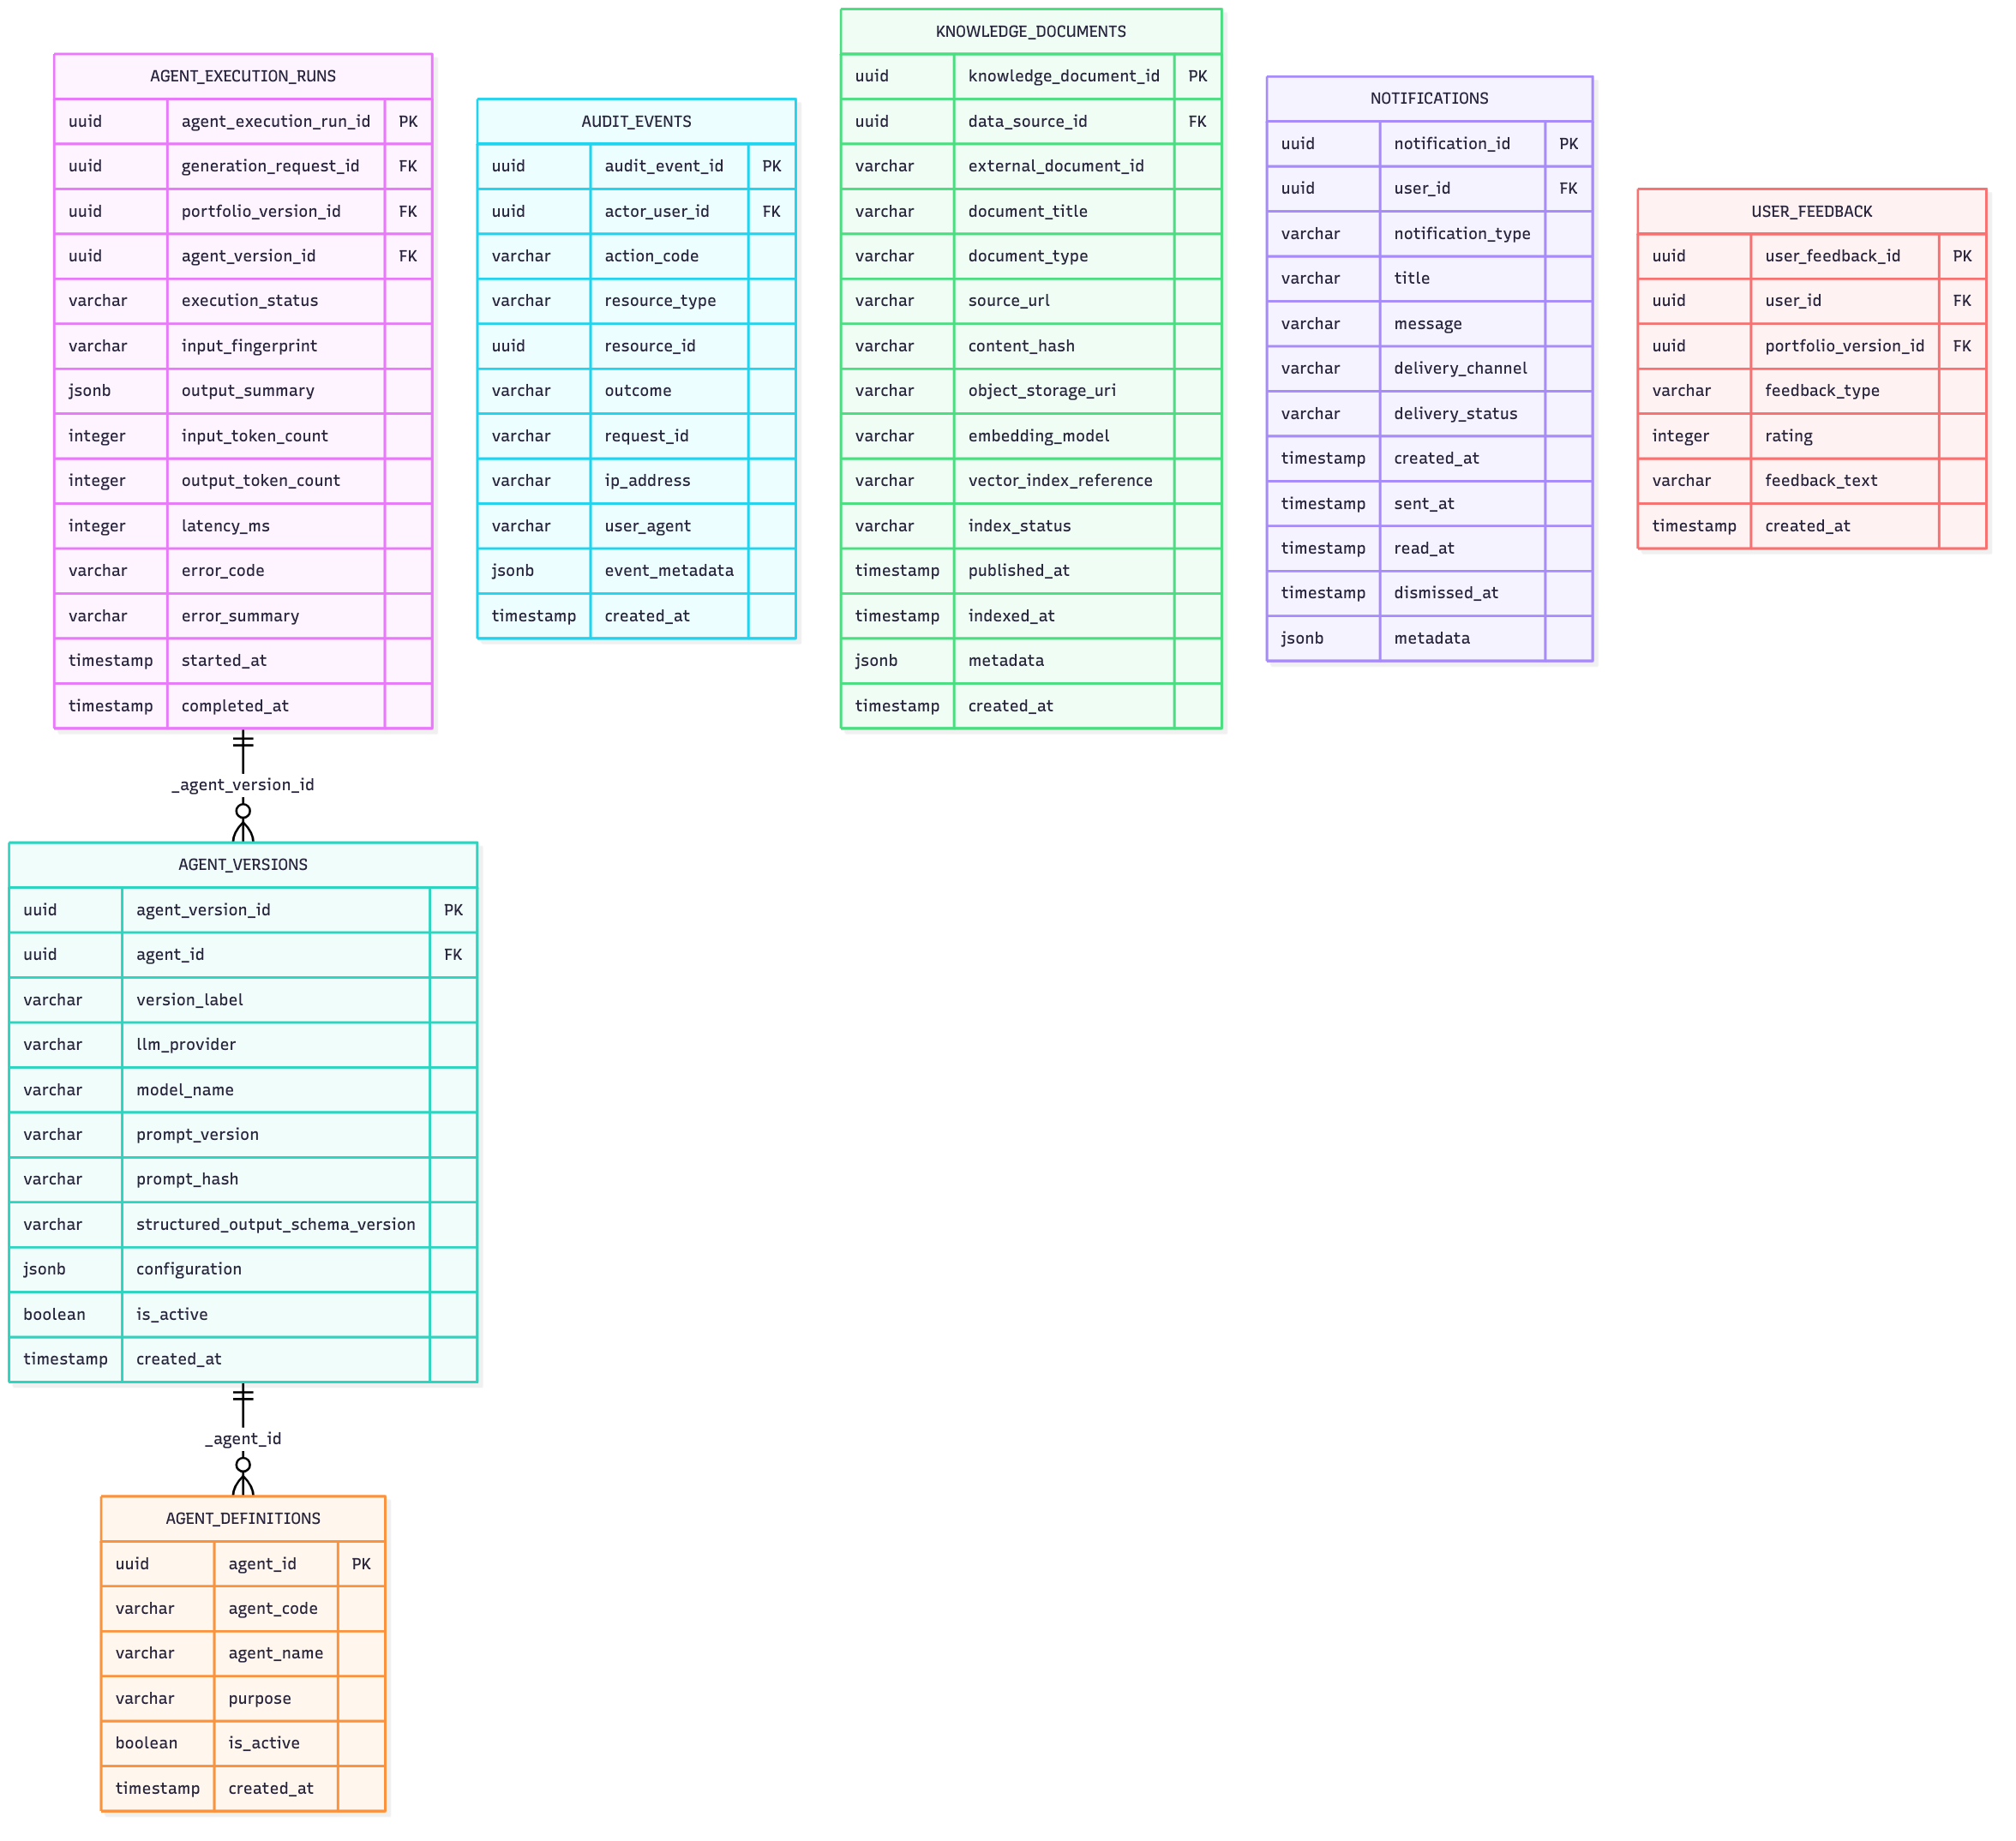
\includegraphics[width=0.88\textwidth, height=0.50\textheight, keepaspectratio]{08_multi_agent_telemetry_and_auditing_domain.png}
    \caption{Domain 8 ER Diagram: Multi-Agent AI Telemetry, Reasoning Traces and Verification}
    \label{fig:er_domain8}
\end{figure}

\section{Database Design Decisions and Performance Optimization}
\begin{enumerate}
    \item \textbf{Normalization vs Performance}: The core operational ledgers (\texttt{app\_users}, \texttt{investor\_portfolios}, \texttt{securities}, \texttt{market\_prices}) are strictly normalized to Third Normal Form (3NF) to eliminate update anomalies. Performance snapshots and diagnostic reports utilize denormalized JSONB columns (\texttt{sector\_skews\_json}, \texttt{factor\_scores\_json}) to facilitate sub-5ms retrieval for frontend dashboard rendering.
    \item \textbf{UUID Primary Keys}: All user, portfolio, and transaction records utilize RFC 4122 Version 4 UUIDs (\texttt{UUID}). This prevents sequential enumeration attacks and facilitates distributed microservice scaling.
    \item \textbf{Indexing Strategy}: High-throughput search columns (\texttt{securities.isin}, \texttt{instrument\_listings.ticker\_symbol}, \texttt{market\_prices.(security\_id, price\_date)}) are supported by B-Tree composite indexes. Text search for stock screening leverages PostgreSQL GIN (Generalized Inverted Index) trgm indexes.
    \item \textbf{Referential Integrity and Cascades}: Strong foreign key constraints safeguard financial ledgers. Deleting a portfolio version automatically cascades to dependent allocations (\texttt{portfolio\_security\_decisions}), while master security and user records enforce \texttt{ON DELETE RESTRICT} to prevent accidental loss of historical transaction ledgers.
\end{enumerate}
